\documentclass[twoside]{book}

% Packages required by doxygen
\usepackage{fixltx2e}
\usepackage{calc}
\usepackage{doxygen}
\usepackage[export]{adjustbox} % also loads graphicx
\usepackage{graphicx}
\usepackage[utf8]{inputenc}
\usepackage{makeidx}
\usepackage{multicol}
\usepackage{multirow}
\PassOptionsToPackage{warn}{textcomp}
\usepackage{textcomp}
\usepackage[nointegrals]{wasysym}
\usepackage[table]{xcolor}

% Font selection
\usepackage[T1]{fontenc}
\usepackage[scaled=.90]{helvet}
\usepackage{courier}
\usepackage{amssymb}
\usepackage{sectsty}
\renewcommand{\familydefault}{\sfdefault}
\allsectionsfont{%
  \fontseries{bc}\selectfont%
  \color{darkgray}%
}
\renewcommand{\DoxyLabelFont}{%
  \fontseries{bc}\selectfont%
  \color{darkgray}%
}
\newcommand{\+}{\discretionary{\mbox{\scriptsize$\hookleftarrow$}}{}{}}

% Page & text layout
\usepackage{geometry}
\geometry{%
  a4paper,%
  top=2.5cm,%
  bottom=2.5cm,%
  left=2.5cm,%
  right=2.5cm%
}
\tolerance=750
\hfuzz=15pt
\hbadness=750
\setlength{\emergencystretch}{15pt}
\setlength{\parindent}{0cm}
\setlength{\parskip}{3ex plus 2ex minus 2ex}
\makeatletter
\renewcommand{\paragraph}{%
  \@startsection{paragraph}{4}{0ex}{-1.0ex}{1.0ex}{%
    \normalfont\normalsize\bfseries\SS@parafont%
  }%
}
\renewcommand{\subparagraph}{%
  \@startsection{subparagraph}{5}{0ex}{-1.0ex}{1.0ex}{%
    \normalfont\normalsize\bfseries\SS@subparafont%
  }%
}
\makeatother

% Headers & footers
\usepackage{fancyhdr}
\pagestyle{fancyplain}
\fancyhead[LE]{\fancyplain{}{\bfseries\thepage}}
\fancyhead[CE]{\fancyplain{}{}}
\fancyhead[RE]{\fancyplain{}{\bfseries\leftmark}}
\fancyhead[LO]{\fancyplain{}{\bfseries\rightmark}}
\fancyhead[CO]{\fancyplain{}{}}
\fancyhead[RO]{\fancyplain{}{\bfseries\thepage}}
\fancyfoot[LE]{\fancyplain{}{}}
\fancyfoot[CE]{\fancyplain{}{}}
\fancyfoot[RE]{\fancyplain{}{\bfseries\scriptsize Generated by Doxygen }}
\fancyfoot[LO]{\fancyplain{}{\bfseries\scriptsize Generated by Doxygen }}
\fancyfoot[CO]{\fancyplain{}{}}
\fancyfoot[RO]{\fancyplain{}{}}
\renewcommand{\footrulewidth}{0.4pt}
\renewcommand{\chaptermark}[1]{%
  \markboth{#1}{}%
}
\renewcommand{\sectionmark}[1]{%
  \markright{\thesection\ #1}%
}

% Indices & bibliography
\usepackage{natbib}
\usepackage[titles]{tocloft}
\setcounter{tocdepth}{3}
\setcounter{secnumdepth}{5}
\makeindex

% Hyperlinks (required, but should be loaded last)
\usepackage{ifpdf}
\ifpdf
  \usepackage[pdftex,pagebackref=true]{hyperref}
\else
  \usepackage[ps2pdf,pagebackref=true]{hyperref}
\fi
\hypersetup{%
  colorlinks=true,%
  linkcolor=blue,%
  citecolor=blue,%
  unicode%
}

% Custom commands
\newcommand{\clearemptydoublepage}{%
  \newpage{\pagestyle{empty}\cleardoublepage}%
}

\usepackage{caption}
\captionsetup{labelsep=space,justification=centering,font={bf},singlelinecheck=off,skip=4pt,position=top}

%===== C O N T E N T S =====

\begin{document}

% Titlepage & ToC
\hypersetup{pageanchor=false,
             bookmarksnumbered=true,
             pdfencoding=unicode
            }
\pagenumbering{alph}
\begin{titlepage}
\vspace*{7cm}
\begin{center}%
{\Large Computer Graphics I -\/ Second Assignment }\\
\vspace*{1cm}
{\large Generated by Doxygen 1.8.13}\\
\end{center}
\end{titlepage}
\clearemptydoublepage
\pagenumbering{roman}
\tableofcontents
\clearemptydoublepage
\pagenumbering{arabic}
\hypersetup{pageanchor=true}

%--- Begin generated contents ---
\chapter{Namespace Index}
\section{Packages}
Here are the packages with brief descriptions (if available)\+:\begin{DoxyCompactList}
\item\contentsline{section}{\hyperlink{namespaceadditional__classes}{additional\+\_\+classes} \\*Extra classes created to extend or complement the other modules }{\pageref{namespaceadditional__classes}}{}
\item\contentsline{section}{\hyperlink{namespacegeometry}{geometry} \\*Classes and geometric utilities commonly used in computational geometry, such as\+: point, line, polygon, triangle and box }{\pageref{namespacegeometry}}{}
\item\contentsline{section}{\hyperlink{namespacemain}{main} \\*The main function, where all the critical parts of the implementation are }{\pageref{namespacemain}}{}
\item\contentsline{section}{\hyperlink{namespacematrix}{matrix} \\*Open\+GL is column major and numpy row major }{\pageref{namespacematrix}}{}
\item\contentsline{section}{\hyperlink{namespacetessellator}{tessellator} \\*Module responsible for utilizing the G\+LU Tessellator }{\pageref{namespacetessellator}}{}
\end{DoxyCompactList}

\chapter{Hierarchical Index}
\section{Class Hierarchy}
This inheritance list is sorted roughly, but not completely, alphabetically\+:\begin{DoxyCompactList}
\item object\begin{DoxyCompactList}
\item \contentsline{section}{additional\+\_\+classes.\+Double\+Click}{\pageref{classadditional__classes_1_1DoubleClick}}{}
\item \contentsline{section}{geometry.\+Box}{\pageref{classgeometry_1_1Box}}{}
\item \contentsline{section}{geometry.\+Line}{\pageref{classgeometry_1_1Line}}{}
\item \contentsline{section}{geometry.\+Point}{\pageref{classgeometry_1_1Point}}{}
\item \contentsline{section}{geometry.\+Polygon}{\pageref{classgeometry_1_1Polygon}}{}
\begin{DoxyCompactList}
\item \contentsline{section}{additional\+\_\+classes.\+Colored\+Polygon}{\pageref{classadditional__classes_1_1ColoredPolygon}}{}
\item \contentsline{section}{geometry.\+Triangle}{\pageref{classgeometry_1_1Triangle}}{}
\end{DoxyCompactList}
\end{DoxyCompactList}
\item \contentsline{section}{additional\+\_\+classes.\+Temporary\+Line}{\pageref{classadditional__classes_1_1TemporaryLine}}{}
\end{DoxyCompactList}

\chapter{Class Index}
\section{Class List}
Here are the classes, structs, unions and interfaces with brief descriptions\+:\begin{DoxyCompactList}
\item\contentsline{section}{\hyperlink{classgeometry_1_1Box}{geometry.\+Box} \\*A bounging box is the smallest rectangle, aligned with the coordinate axes, which contain a given set of points }{\pageref{classgeometry_1_1Box}}{}
\item\contentsline{section}{\hyperlink{classadditional__classes_1_1ColoredPolygon}{additional\+\_\+classes.\+Colored\+Polygon} \\*Class that extends the Polygon class from the geometry module }{\pageref{classadditional__classes_1_1ColoredPolygon}}{}
\item\contentsline{section}{\hyperlink{classadditional__classes_1_1DoubleClick}{additional\+\_\+classes.\+Double\+Click} \\*Class that implements the double click logic, used to place the nails }{\pageref{classadditional__classes_1_1DoubleClick}}{}
\item\contentsline{section}{\hyperlink{classgeometry_1_1Line}{geometry.\+Line} \\*Two points define a straight line }{\pageref{classgeometry_1_1Line}}{}
\item\contentsline{section}{\hyperlink{classgeometry_1_1Point}{geometry.\+Point} \\*Implements a 3D point or vector }{\pageref{classgeometry_1_1Point}}{}
\item\contentsline{section}{\hyperlink{classgeometry_1_1Polygon}{geometry.\+Polygon} \\*In elementary geometry, a polygon is a plane figure that is bounded by a finite chain of straight line segments, closing in a loop, to form a closed polygonal chain or circuit }{\pageref{classgeometry_1_1Polygon}}{}
\item\contentsline{section}{\hyperlink{classadditional__classes_1_1TemporaryLine}{additional\+\_\+classes.\+Temporary\+Line} \\*Class that defines a temporary line (used to draw the temporary lines representing the polygon edges) }{\pageref{classadditional__classes_1_1TemporaryLine}}{}
\item\contentsline{section}{\hyperlink{classgeometry_1_1Triangle}{geometry.\+Triangle} \\*A triangle is a polygon with three edges and three vertices }{\pageref{classgeometry_1_1Triangle}}{}
\end{DoxyCompactList}

\chapter{Namespace Documentation}
\hypertarget{namespaceadditional__classes}{}\section{additional\+\_\+classes Namespace Reference}
\label{namespaceadditional__classes}\index{additional\+\_\+classes@{additional\+\_\+classes}}


Extra classes created to extend or complement the other modules.  


\subsection*{Classes}
\begin{DoxyCompactItemize}
\item 
class \hyperlink{classadditional__classes_1_1ColoredPolygon}{Colored\+Polygon}
\begin{DoxyCompactList}\small\item\em Class that extends the Polygon class from the geometry module. \end{DoxyCompactList}\item 
class \hyperlink{classadditional__classes_1_1DoubleClick}{Double\+Click}
\begin{DoxyCompactList}\small\item\em Class that implements the double click logic, used to place the nails. \end{DoxyCompactList}\item 
class \hyperlink{classadditional__classes_1_1TemporaryLine}{Temporary\+Line}
\begin{DoxyCompactList}\small\item\em Class that defines a temporary line (used to draw the temporary lines representing the polygon edges) \end{DoxyCompactList}\end{DoxyCompactItemize}


\subsection{Detailed Description}
Extra classes created to extend or complement the other modules. 

\begin{DoxyAuthor}{Author}
Lucas Rodrigues 
\end{DoxyAuthor}

\hypertarget{namespacegeometry}{}\section{geometry Namespace Reference}
\label{namespacegeometry}\index{geometry@{geometry}}


Classes and geometric utilities commonly used in computational geometry, such as\+: point, line, polygon, triangle and box.  


\subsection*{Classes}
\begin{DoxyCompactItemize}
\item 
class \hyperlink{classgeometry_1_1Box}{Box}
\begin{DoxyCompactList}\small\item\em A bounging box is the smallest rectangle, aligned with the coordinate axes, which contain a given set of points. \end{DoxyCompactList}\item 
class \hyperlink{classgeometry_1_1Line}{Line}
\begin{DoxyCompactList}\small\item\em Two points define a straight line. \end{DoxyCompactList}\item 
class \hyperlink{classgeometry_1_1Point}{Point}
\begin{DoxyCompactList}\small\item\em Implements a 3D point or vector. \end{DoxyCompactList}\item 
class \hyperlink{classgeometry_1_1Polygon}{Polygon}
\begin{DoxyCompactList}\small\item\em In elementary geometry, a polygon is a plane figure that is bounded by a finite chain of straight line segments, closing in a loop, to form a closed polygonal chain or circuit. \end{DoxyCompactList}\item 
class \hyperlink{classgeometry_1_1Triangle}{Triangle}
\begin{DoxyCompactList}\small\item\em A triangle is a polygon with three edges and three vertices. \end{DoxyCompactList}\end{DoxyCompactItemize}
\subsection*{Functions}
\begin{DoxyCompactItemize}
\item 
def \hyperlink{namespacegeometry_a826edf3113b2277f596bc7927da2fd4e}{ccw3} (A, B, C, N)
\item 
def \hyperlink{namespacegeometry_ad67511f31b70990660efd63da577f482}{ccw} (A, B, C)
\item 
def \hyperlink{namespacegeometry_a3df8ee137b8d01576f14084dee3a6a91}{intersect} (a1, b1, a2, b2)
\item 
def \hyperlink{namespacegeometry_a118331eb1c38459dd57dad62f75abea5}{close} (a, b, epsilon=\hyperlink{namespacegeometry_a543db87a5e9af9e1d17146559a540276}{E\+PS})
\item 
def \hyperlink{namespacegeometry_acaccff5b694d39c9db5072c671c6568b}{shortest\+Path\+To\+Line} (self, that)
\begin{DoxyCompactList}\small\item\em Calculate the line segment Pa\+Pb that is the shortest route between two lines P1\+P2 and P3\+P4. \end{DoxyCompactList}\item 
def \hyperlink{namespacegeometry_a96071e09708da91677cc86ea91705f5e}{distance\+To\+Line} (self, that)
\item 
def \hyperlink{namespacegeometry_afe255f1239fc866c1c2c04b30c37b696}{intersection} (self, that)
\item 
def \hyperlink{namespacegeometry_aa7e72b904b344b7d45b75f3942bc618b}{midpoint} (self)
\item 
def \hyperlink{namespacegeometry_a08506b08fe50ecd6e3c7098f63178881}{intersect\+To\+Plane} (self, poly)
\item 
def \hyperlink{namespacegeometry_a7c89848bc4970d590b82641648503bd9}{area} (self)
\begin{DoxyCompactList}\small\item\em Calculates the area of a planar polygon. \end{DoxyCompactList}\item 
def \hyperlink{namespacegeometry_a9453ec6bad9d4ba50724a4df0b1a74ed}{distance} (self, p)
\begin{DoxyCompactList}\small\item\em Returns the distance of a given point to the plane of this polygon. \end{DoxyCompactList}\item 
def \hyperlink{namespacegeometry_ac7327d8cae2a771c06a0ded4c91ab4a7}{interior\+Point} (self)
\item 
def \hyperlink{namespacegeometry_ac3bf912ad06b884d2c21a3f91cf7c392}{exterior\+Point} (self)
\item 
def \hyperlink{namespacegeometry_a284499afed4bfe4096ca1c78062a16bb}{main} ()
\end{DoxyCompactItemize}
\subsection*{Variables}
\begin{DoxyCompactItemize}
\item 
float \hyperlink{namespacegeometry_a543db87a5e9af9e1d17146559a540276}{E\+PS} = 0.\+001
\begin{DoxyCompactList}\small\item\em Tolerance used for checking equalities. \end{DoxyCompactList}\end{DoxyCompactItemize}


\subsection{Detailed Description}
Classes and geometric utilities commonly used in computational geometry, such as\+: point, line, polygon, triangle and box. 

\begin{DoxyAuthor}{Author}
Flavia Cavalcanti 
\end{DoxyAuthor}
\begin{DoxyDate}{Date}
01/02/2017 
\end{DoxyDate}


\subsection{Function Documentation}
\mbox{\Hypertarget{namespacegeometry_a7c89848bc4970d590b82641648503bd9}\label{namespacegeometry_a7c89848bc4970d590b82641648503bd9}} 
\index{geometry@{geometry}!area@{area}}
\index{area@{area}!geometry@{geometry}}
\subsubsection{\texorpdfstring{area()}{area()}}
{\footnotesize\ttfamily def geometry.\+area (\begin{DoxyParamCaption}\item[{}]{self }\end{DoxyParamCaption})}



Calculates the area of a planar polygon. 

The algorithm is as follows\+:~\newline
 \begin{DoxyVerb}Traverse the loop of coordinates, assuming that it is in
clockwise order, computing the components of the "area" of the
enclosed polygon.  The total "area" components are computed by
adding "area" components (cross product components) of
triangles sides formed by the first, previous, and current
vertices.  If the loop is not convex, some of the triangle
areas might be negative, but those will be compensated by other
positive triangle areas so that the final area is positive.<br>
\end{DoxyVerb}


Note\+: area here is actually twice the area. ~\newline
 positive here means in the direction of the face normal.

\begin{DoxyReturn}{Returns}
twice the polygon area.\begin{DoxyVerb}Returns the area of the polygon.\end{DoxyVerb}
 
\end{DoxyReturn}


Definition at line 475 of file geometry.\+py.

\mbox{\Hypertarget{namespacegeometry_ad67511f31b70990660efd63da577f482}\label{namespacegeometry_ad67511f31b70990660efd63da577f482}} 
\index{geometry@{geometry}!ccw@{ccw}}
\index{ccw@{ccw}!geometry@{geometry}}
\subsubsection{\texorpdfstring{ccw()}{ccw()}}
{\footnotesize\ttfamily def geometry.\+ccw (\begin{DoxyParamCaption}\item[{}]{A,  }\item[{}]{B,  }\item[{}]{C }\end{DoxyParamCaption})}

\begin{DoxyVerb}Tests whether the angle formed by 2D points A, B, and C is ccw.\end{DoxyVerb}
 

Definition at line 23 of file geometry.\+py.

\mbox{\Hypertarget{namespacegeometry_a826edf3113b2277f596bc7927da2fd4e}\label{namespacegeometry_a826edf3113b2277f596bc7927da2fd4e}} 
\index{geometry@{geometry}!ccw3@{ccw3}}
\index{ccw3@{ccw3}!geometry@{geometry}}
\subsubsection{\texorpdfstring{ccw3()}{ccw3()}}
{\footnotesize\ttfamily def geometry.\+ccw3 (\begin{DoxyParamCaption}\item[{}]{A,  }\item[{}]{B,  }\item[{}]{C,  }\item[{}]{N }\end{DoxyParamCaption})}

\begin{DoxyVerb}Tests whether the angle formed by 3D points A, B, C and normal N is ccw.\end{DoxyVerb}
 

Definition at line 19 of file geometry.\+py.

\mbox{\Hypertarget{namespacegeometry_a118331eb1c38459dd57dad62f75abea5}\label{namespacegeometry_a118331eb1c38459dd57dad62f75abea5}} 
\index{geometry@{geometry}!close@{close}}
\index{close@{close}!geometry@{geometry}}
\subsubsection{\texorpdfstring{close()}{close()}}
{\footnotesize\ttfamily def geometry.\+close (\begin{DoxyParamCaption}\item[{}]{a,  }\item[{}]{b,  }\item[{}]{epsilon = {\ttfamily \hyperlink{namespacegeometry_a543db87a5e9af9e1d17146559a540276}{E\+PS}} }\end{DoxyParamCaption})}

\begin{DoxyVerb}Returns whether two floats a and b are equal.\end{DoxyVerb}
 

Definition at line 32 of file geometry.\+py.

\mbox{\Hypertarget{namespacegeometry_a9453ec6bad9d4ba50724a4df0b1a74ed}\label{namespacegeometry_a9453ec6bad9d4ba50724a4df0b1a74ed}} 
\index{geometry@{geometry}!distance@{distance}}
\index{distance@{distance}!geometry@{geometry}}
\subsubsection{\texorpdfstring{distance()}{distance()}}
{\footnotesize\ttfamily def geometry.\+distance (\begin{DoxyParamCaption}\item[{}]{self,  }\item[{}]{p }\end{DoxyParamCaption})}



Returns the distance of a given point to the plane of this polygon. 

\begin{DoxyReturn}{Returns}
dist(p) = 0, if p is onto the plane, $>$ 0, if p is into the semi-\/space pointed to by the normal vector, $<$ 0, otherwise.
\end{DoxyReturn}
\begin{DoxySeeAlso}{See also}
\href{http://mathinsight.org/distance_point_plane@verbatim}{\tt http\+://mathinsight.\+org/distance\+\_\+point\+\_\+plane@verbatim} "Returns the \hyperlink{namespacegeometry_a9453ec6bad9d4ba50724a4df0b1a74ed}{distance} of a given point to the plane of this polygon. 
\end{DoxySeeAlso}


Definition at line 496 of file geometry.\+py.

\mbox{\Hypertarget{namespacegeometry_a96071e09708da91677cc86ea91705f5e}\label{namespacegeometry_a96071e09708da91677cc86ea91705f5e}} 
\index{geometry@{geometry}!distance\+To\+Line@{distance\+To\+Line}}
\index{distance\+To\+Line@{distance\+To\+Line}!geometry@{geometry}}
\subsubsection{\texorpdfstring{distance\+To\+Line()}{distanceToLine()}}
{\footnotesize\ttfamily def geometry.\+distance\+To\+Line (\begin{DoxyParamCaption}\item[{}]{self,  }\item[{}]{that }\end{DoxyParamCaption})}

\begin{DoxyVerb}Returns the distance between two lines.\end{DoxyVerb}
 

Definition at line 299 of file geometry.\+py.

\mbox{\Hypertarget{namespacegeometry_ac3bf912ad06b884d2c21a3f91cf7c392}\label{namespacegeometry_ac3bf912ad06b884d2c21a3f91cf7c392}} 
\index{geometry@{geometry}!exterior\+Point@{exterior\+Point}}
\index{exterior\+Point@{exterior\+Point}!geometry@{geometry}}
\subsubsection{\texorpdfstring{exterior\+Point()}{exteriorPoint()}}
{\footnotesize\ttfamily def geometry.\+exterior\+Point (\begin{DoxyParamCaption}\item[{}]{self }\end{DoxyParamCaption})}

\begin{DoxyVerb}Returns a random exterior point near the polygon.\end{DoxyVerb}
 

Definition at line 523 of file geometry.\+py.

\mbox{\Hypertarget{namespacegeometry_ac7327d8cae2a771c06a0ded4c91ab4a7}\label{namespacegeometry_ac7327d8cae2a771c06a0ded4c91ab4a7}} 
\index{geometry@{geometry}!interior\+Point@{interior\+Point}}
\index{interior\+Point@{interior\+Point}!geometry@{geometry}}
\subsubsection{\texorpdfstring{interior\+Point()}{interiorPoint()}}
{\footnotesize\ttfamily def geometry.\+interior\+Point (\begin{DoxyParamCaption}\item[{}]{self }\end{DoxyParamCaption})}

\begin{DoxyVerb}Returns a random interior point via rejection sampling.\end{DoxyVerb}
 

Definition at line 505 of file geometry.\+py.

\mbox{\Hypertarget{namespacegeometry_a3df8ee137b8d01576f14084dee3a6a91}\label{namespacegeometry_a3df8ee137b8d01576f14084dee3a6a91}} 
\index{geometry@{geometry}!intersect@{intersect}}
\index{intersect@{intersect}!geometry@{geometry}}
\subsubsection{\texorpdfstring{intersect()}{intersect()}}
{\footnotesize\ttfamily def geometry.\+intersect (\begin{DoxyParamCaption}\item[{}]{a1,  }\item[{}]{b1,  }\item[{}]{a2,  }\item[{}]{b2 }\end{DoxyParamCaption})}

\begin{DoxyVerb}Returns True if the line segments a1b1 and a2b2 intersect.\end{DoxyVerb}
 

Definition at line 27 of file geometry.\+py.

\mbox{\Hypertarget{namespacegeometry_afe255f1239fc866c1c2c04b30c37b696}\label{namespacegeometry_afe255f1239fc866c1c2c04b30c37b696}} 
\index{geometry@{geometry}!intersection@{intersection}}
\index{intersection@{intersection}!geometry@{geometry}}
\subsubsection{\texorpdfstring{intersection()}{intersection()}}
{\footnotesize\ttfamily def geometry.\+intersection (\begin{DoxyParamCaption}\item[{}]{self,  }\item[{}]{that }\end{DoxyParamCaption})}

\begin{DoxyVerb}Returns the intersection point between two lines.\end{DoxyVerb}
 

Definition at line 308 of file geometry.\+py.

\mbox{\Hypertarget{namespacegeometry_a08506b08fe50ecd6e3c7098f63178881}\label{namespacegeometry_a08506b08fe50ecd6e3c7098f63178881}} 
\index{geometry@{geometry}!intersect\+To\+Plane@{intersect\+To\+Plane}}
\index{intersect\+To\+Plane@{intersect\+To\+Plane}!geometry@{geometry}}
\subsubsection{\texorpdfstring{intersect\+To\+Plane()}{intersectToPlane()}}
{\footnotesize\ttfamily def geometry.\+intersect\+To\+Plane (\begin{DoxyParamCaption}\item[{}]{self,  }\item[{}]{poly }\end{DoxyParamCaption})}

\begin{DoxyVerb}Returns the intersection between this line and a given polygon plane.\end{DoxyVerb}
 

Definition at line 325 of file geometry.\+py.

\mbox{\Hypertarget{namespacegeometry_a284499afed4bfe4096ca1c78062a16bb}\label{namespacegeometry_a284499afed4bfe4096ca1c78062a16bb}} 
\index{geometry@{geometry}!main@{main}}
\index{main@{main}!geometry@{geometry}}
\subsubsection{\texorpdfstring{main()}{main()}}
{\footnotesize\ttfamily def geometry.\+main (\begin{DoxyParamCaption}{ }\end{DoxyParamCaption})}

\begin{DoxyVerb}Main program for testing.\end{DoxyVerb}
 

Definition at line 686 of file geometry.\+py.

\mbox{\Hypertarget{namespacegeometry_aa7e72b904b344b7d45b75f3942bc618b}\label{namespacegeometry_aa7e72b904b344b7d45b75f3942bc618b}} 
\index{geometry@{geometry}!midpoint@{midpoint}}
\index{midpoint@{midpoint}!geometry@{geometry}}
\subsubsection{\texorpdfstring{midpoint()}{midpoint()}}
{\footnotesize\ttfamily def geometry.\+midpoint (\begin{DoxyParamCaption}\item[{}]{self }\end{DoxyParamCaption})}

\begin{DoxyVerb}Returns the middle point of this segment.\end{DoxyVerb}
 

Definition at line 317 of file geometry.\+py.

\mbox{\Hypertarget{namespacegeometry_acaccff5b694d39c9db5072c671c6568b}\label{namespacegeometry_acaccff5b694d39c9db5072c671c6568b}} 
\index{geometry@{geometry}!shortest\+Path\+To\+Line@{shortest\+Path\+To\+Line}}
\index{shortest\+Path\+To\+Line@{shortest\+Path\+To\+Line}!geometry@{geometry}}
\subsubsection{\texorpdfstring{shortest\+Path\+To\+Line()}{shortestPathToLine()}}
{\footnotesize\ttfamily def geometry.\+shortest\+Path\+To\+Line (\begin{DoxyParamCaption}\item[{}]{self,  }\item[{}]{that }\end{DoxyParamCaption})}



Calculate the line segment Pa\+Pb that is the shortest route between two lines P1\+P2 and P3\+P4. 

Calculate also the values of mua and mub where Pa = P1 + mua (P2 -\/ P1) Pb = P3 + mub (P4 -\/ P3) Return None if no solution exists.\begin{DoxyVerb}Return the shortest segment between two lines.

   @see http://paulbourke.net/geometry/pointlineplane/
\end{DoxyVerb}
 

Definition at line 255 of file geometry.\+py.



\subsection{Variable Documentation}
\mbox{\Hypertarget{namespacegeometry_a543db87a5e9af9e1d17146559a540276}\label{namespacegeometry_a543db87a5e9af9e1d17146559a540276}} 
\index{geometry@{geometry}!E\+PS@{E\+PS}}
\index{E\+PS@{E\+PS}!geometry@{geometry}}
\subsubsection{\texorpdfstring{E\+PS}{EPS}}
{\footnotesize\ttfamily float geometry.\+E\+PS = 0.\+001}



Tolerance used for checking equalities. 



Definition at line 17 of file geometry.\+py.


\hypertarget{namespacemain}{}\section{main Namespace Reference}
\label{namespacemain}\index{main@{main}}


The main function, where all the critical parts of the implementation are.  


\subsection*{Functions}
\begin{DoxyCompactItemize}
\item 
def \hyperlink{namespacemain_a526cfe84f4e80095febf0d3f4b7b5358}{change\+Size} (w, h)
\begin{DoxyCompactList}\small\item\em Function to resize the window. \end{DoxyCompactList}\item 
def \hyperlink{namespacemain_a88fcd4aa7193703d53a8095e78a40fe9}{can\+Translate} (polygon, children)
\begin{DoxyCompactList}\small\item\em Function that determines whether if a polygon can be translated based on its position in the hierarchy. \end{DoxyCompactList}\item 
def \hyperlink{namespacemain_ae1d466859928a06baa89a7b9279f4fa1}{can\+Rotate} (polygon)
\begin{DoxyCompactList}\small\item\em Function that determines whether if a polygon can be rotated based on its position in the hierarchy. \end{DoxyCompactList}\item 
def \hyperlink{namespacemain_a0f7b954a9ec1b9e21e5d888e630d1ed0}{my\+Mouse} (button, state, x, y)
\begin{DoxyCompactList}\small\item\em Callback function to handle mouse input. \end{DoxyCompactList}\item 
\mbox{\Hypertarget{namespacemain_a9641b8c073c7079e597f39b5f7f6cf0d}\label{namespacemain_a9641b8c073c7079e597f39b5f7f6cf0d}} 
def \hyperlink{namespacemain_a9641b8c073c7079e597f39b5f7f6cf0d}{cancel\+Polygon} ()
\begin{DoxyCompactList}\small\item\em Function that cancels the polygon that is being currently drawn. \end{DoxyCompactList}\item 
def \hyperlink{namespacemain_abfe7963151804b73036937ad486f55ac}{rotate\+Polygon} (point)
\begin{DoxyCompactList}\small\item\em Function that rotates a polygon using the given point as axis. \end{DoxyCompactList}\item 
def \hyperlink{namespacemain_adeb2cd76f03836777dd43cb9bc133d89}{translate\+Polygon} (polygon, point)
\begin{DoxyCompactList}\small\item\em Function that translates the polygon to a point of destination. \end{DoxyCompactList}\item 
def \hyperlink{namespacemain_aeae47c61066756f699b19bf97f937370}{apply\+Transformation\+To\+Children} (polygon, matrix)
\begin{DoxyCompactList}\small\item\em Function that applies transformations to their children in the hierarchy. \end{DoxyCompactList}\item 
def \hyperlink{namespacemain_a69cc12fb1c27fecdfcac61f5d4e917b9}{apply\+Transformation\+To\+Points} (polygon, matrix)
\begin{DoxyCompactList}\small\item\em Function that applies the transformation to points (nails) \end{DoxyCompactList}\item 
def \hyperlink{namespacemain_afa0ac21cfc8ed3c2c3cfddd6ea6899b6}{intersects} (l1, l2)
\begin{DoxyCompactList}\small\item\em Function that checks whether two lines intersect. \end{DoxyCompactList}\item 
def \hyperlink{namespacemain_aac29b4e8c9fa3c64c062e76290492fb8}{mouse\+Motion} (x, y)
\begin{DoxyCompactList}\small\item\em Callback function used to monitor the mouse motion while clicked. \end{DoxyCompactList}\item 
def \hyperlink{namespacemain_a33eac5e1e174927a801f847ff8c2d484}{mouse\+Drag} (x, y)
\begin{DoxyCompactList}\small\item\em Callback function that passively monitors mouse motion. \end{DoxyCompactList}\item 
\mbox{\Hypertarget{namespacemain_aa9279d9a799d74c5bf21beff5da0062a}\label{namespacemain_aa9279d9a799d74c5bf21beff5da0062a}} 
def \hyperlink{namespacemain_aa9279d9a799d74c5bf21beff5da0062a}{draw\+Temp\+Lines} ()
\begin{DoxyCompactList}\small\item\em Function that draws the temporary lines that represent the polygon edges. \end{DoxyCompactList}\item 
def \hyperlink{namespacemain_a923e8cecbed43bf133611a409c40c107}{draw\+Polygon} (polygon)
\begin{DoxyCompactList}\small\item\em Function that draws the polygons. \end{DoxyCompactList}\item 
def \hyperlink{namespacemain_a020b084aad026564a4c7ee5af1ac6b91}{draw\+Nails} (polygon)
\begin{DoxyCompactList}\small\item\em Function that draws the nails. \end{DoxyCompactList}\item 
\mbox{\Hypertarget{namespacemain_a9258848a9cd7db8568ec88c7846c4768}\label{namespacemain_a9258848a9cd7db8568ec88c7846c4768}} 
def \hyperlink{namespacemain_a9258848a9cd7db8568ec88c7846c4768}{render\+Scene} ()
\begin{DoxyCompactList}\small\item\em Callback function that renders the scene. \end{DoxyCompactList}\item 
\mbox{\Hypertarget{namespacemain_a23a088b39943d6376eeea956b0afbd48}\label{namespacemain_a23a088b39943d6376eeea956b0afbd48}} 
def \hyperlink{namespacemain_a23a088b39943d6376eeea956b0afbd48}{main} (argv=None)
\begin{DoxyCompactList}\small\item\em Main function. \end{DoxyCompactList}\end{DoxyCompactItemize}
\subsection*{Variables}
\begin{DoxyCompactItemize}
\item 
\mbox{\Hypertarget{namespacemain_a45532432f3eaf99712b1c921e1e7fa96}\label{namespacemain_a45532432f3eaf99712b1c921e1e7fa96}} 
int {\bfseries width} = 800
\item 
\mbox{\Hypertarget{namespacemain_a94be9c33154f8abfadfc37bd3f07d910}\label{namespacemain_a94be9c33154f8abfadfc37bd3f07d910}} 
int {\bfseries height} = 600
\item 
\mbox{\Hypertarget{namespacemain_ad6ed2ca0de7745c0538b39f53443f6fa}\label{namespacemain_ad6ed2ca0de7745c0538b39f53443f6fa}} 
{\bfseries temp\+Line} = \hyperlink{classadditional__classes_1_1TemporaryLine}{Temporary\+Line}(\hyperlink{classgeometry_1_1Point}{Point}(0,0))
\item 
\mbox{\Hypertarget{namespacemain_ac179743eef5260b1b36e9867eeaa459e}\label{namespacemain_ac179743eef5260b1b36e9867eeaa459e}} 
list {\bfseries polygons} = \mbox{[}$\,$\mbox{]}
\item 
\mbox{\Hypertarget{namespacemain_a184193594cc4348fd4f60c39b6a01fcc}\label{namespacemain_a184193594cc4348fd4f60c39b6a01fcc}} 
list {\bfseries nails} = \mbox{[}$\,$\mbox{]}
\item 
\mbox{\Hypertarget{namespacemain_adf37c1088b5a3b0bb91496b491b8a83c}\label{namespacemain_adf37c1088b5a3b0bb91496b491b8a83c}} 
bool {\bfseries clicked} = False
\item 
\mbox{\Hypertarget{namespacemain_a6e44d6dc26cd21cbe7c927f09b7d4d21}\label{namespacemain_a6e44d6dc26cd21cbe7c927f09b7d4d21}} 
list {\bfseries current\+Polygon} = \mbox{[}$\,$\mbox{]}
\item 
\mbox{\Hypertarget{namespacemain_a3642375aa9ef1e3fd8ef4a2cd4c09e8e}\label{namespacemain_a3642375aa9ef1e3fd8ef4a2cd4c09e8e}} 
{\bfseries selected\+Polygon} = None
\item 
\mbox{\Hypertarget{namespacemain_ad8ecf5db937f2635bf56dcdf3385e8e5}\label{namespacemain_ad8ecf5db937f2635bf56dcdf3385e8e5}} 
{\bfseries double\+Click} = \hyperlink{classadditional__classes_1_1DoubleClick}{Double\+Click}(time())
\item 
\mbox{\Hypertarget{namespacemain_a6e5230fd1a746cd13a3cf00f6b50db5a}\label{namespacemain_a6e5230fd1a746cd13a3cf00f6b50db5a}} 
list {\bfseries transformed\+Children} = \mbox{[}$\,$\mbox{]}
\item 
\mbox{\Hypertarget{namespacemain_aef6d673950d75316b45b1d74dc79db40}\label{namespacemain_aef6d673950d75316b45b1d74dc79db40}} 
list {\bfseries transformed\+Nails} = \mbox{[}$\,$\mbox{]}
\end{DoxyCompactItemize}


\subsection{Detailed Description}
The main function, where all the critical parts of the implementation are. 

\begin{DoxyAuthor}{Author}
Lucas Rodrigues 
\end{DoxyAuthor}


\subsection{Function Documentation}
\mbox{\Hypertarget{namespacemain_aeae47c61066756f699b19bf97f937370}\label{namespacemain_aeae47c61066756f699b19bf97f937370}} 
\index{main@{main}!apply\+Transformation\+To\+Children@{apply\+Transformation\+To\+Children}}
\index{apply\+Transformation\+To\+Children@{apply\+Transformation\+To\+Children}!main@{main}}
\subsubsection{\texorpdfstring{apply\+Transformation\+To\+Children()}{applyTransformationToChildren()}}
{\footnotesize\ttfamily def main.\+apply\+Transformation\+To\+Children (\begin{DoxyParamCaption}\item[{}]{polygon,  }\item[{}]{matrix }\end{DoxyParamCaption})}



Function that applies transformations to their children in the hierarchy. 


\begin{DoxyParams}{Parameters}
{\em polygon} & The parent polygon \\
\hline
{\em matrix} & The transformation matrix being applied \\
\hline
\end{DoxyParams}


Definition at line 236 of file main.\+py.

\mbox{\Hypertarget{namespacemain_a69cc12fb1c27fecdfcac61f5d4e917b9}\label{namespacemain_a69cc12fb1c27fecdfcac61f5d4e917b9}} 
\index{main@{main}!apply\+Transformation\+To\+Points@{apply\+Transformation\+To\+Points}}
\index{apply\+Transformation\+To\+Points@{apply\+Transformation\+To\+Points}!main@{main}}
\subsubsection{\texorpdfstring{apply\+Transformation\+To\+Points()}{applyTransformationToPoints()}}
{\footnotesize\ttfamily def main.\+apply\+Transformation\+To\+Points (\begin{DoxyParamCaption}\item[{}]{polygon,  }\item[{}]{matrix }\end{DoxyParamCaption})}



Function that applies the transformation to points (nails) 


\begin{DoxyParams}{Parameters}
{\em polygon} & The polygon which has the nails \\
\hline
{\em matrix} & The transformation matrix being applied \\
\hline
\end{DoxyParams}


Definition at line 246 of file main.\+py.

\mbox{\Hypertarget{namespacemain_ae1d466859928a06baa89a7b9279f4fa1}\label{namespacemain_ae1d466859928a06baa89a7b9279f4fa1}} 
\index{main@{main}!can\+Rotate@{can\+Rotate}}
\index{can\+Rotate@{can\+Rotate}!main@{main}}
\subsubsection{\texorpdfstring{can\+Rotate()}{canRotate()}}
{\footnotesize\ttfamily def main.\+can\+Rotate (\begin{DoxyParamCaption}\item[{}]{polygon }\end{DoxyParamCaption})}



Function that determines whether if a polygon can be rotated based on its position in the hierarchy. 


\begin{DoxyParams}{Parameters}
{\em polygon} & The polygon being tested \\
\hline
\end{DoxyParams}
\begin{DoxyReturn}{Returns}
Returns true if the polygon can be rotated, and False otherwise 
\end{DoxyReturn}


Definition at line 75 of file main.\+py.

\mbox{\Hypertarget{namespacemain_a88fcd4aa7193703d53a8095e78a40fe9}\label{namespacemain_a88fcd4aa7193703d53a8095e78a40fe9}} 
\index{main@{main}!can\+Translate@{can\+Translate}}
\index{can\+Translate@{can\+Translate}!main@{main}}
\subsubsection{\texorpdfstring{can\+Translate()}{canTranslate()}}
{\footnotesize\ttfamily def main.\+can\+Translate (\begin{DoxyParamCaption}\item[{}]{polygon,  }\item[{}]{children }\end{DoxyParamCaption})}



Function that determines whether if a polygon can be translated based on its position in the hierarchy. 


\begin{DoxyParams}{Parameters}
{\em polygon} & The polygon being tested \\
\hline
{\em children} & The list of polygons that are below polygon on the hierarchy \\
\hline
\end{DoxyParams}
\begin{DoxyReturn}{Returns}
Returns true if the polygon can be translated, and False otherwise 
\end{DoxyReturn}


Definition at line 62 of file main.\+py.

\mbox{\Hypertarget{namespacemain_a526cfe84f4e80095febf0d3f4b7b5358}\label{namespacemain_a526cfe84f4e80095febf0d3f4b7b5358}} 
\index{main@{main}!change\+Size@{change\+Size}}
\index{change\+Size@{change\+Size}!main@{main}}
\subsubsection{\texorpdfstring{change\+Size()}{changeSize()}}
{\footnotesize\ttfamily def main.\+change\+Size (\begin{DoxyParamCaption}\item[{}]{w,  }\item[{}]{h }\end{DoxyParamCaption})}



Function to resize the window. 


\begin{DoxyParams}{Parameters}
{\em w} & The screen width \\
\hline
{\em h} & The screen height \\
\hline
\end{DoxyParams}


Definition at line 37 of file main.\+py.

\mbox{\Hypertarget{namespacemain_a020b084aad026564a4c7ee5af1ac6b91}\label{namespacemain_a020b084aad026564a4c7ee5af1ac6b91}} 
\index{main@{main}!draw\+Nails@{draw\+Nails}}
\index{draw\+Nails@{draw\+Nails}!main@{main}}
\subsubsection{\texorpdfstring{draw\+Nails()}{drawNails()}}
{\footnotesize\ttfamily def main.\+draw\+Nails (\begin{DoxyParamCaption}\item[{}]{polygon }\end{DoxyParamCaption})}



Function that draws the nails. 


\begin{DoxyParams}{Parameters}
{\em polygon} & The polygon which has nails associated to it \\
\hline
\end{DoxyParams}


Definition at line 338 of file main.\+py.

\mbox{\Hypertarget{namespacemain_a923e8cecbed43bf133611a409c40c107}\label{namespacemain_a923e8cecbed43bf133611a409c40c107}} 
\index{main@{main}!draw\+Polygon@{draw\+Polygon}}
\index{draw\+Polygon@{draw\+Polygon}!main@{main}}
\subsubsection{\texorpdfstring{draw\+Polygon()}{drawPolygon()}}
{\footnotesize\ttfamily def main.\+draw\+Polygon (\begin{DoxyParamCaption}\item[{}]{polygon }\end{DoxyParamCaption})}



Function that draws the polygons. 


\begin{DoxyParams}{Parameters}
{\em polygon} & The polygon being drawn \\
\hline
\end{DoxyParams}


Definition at line 331 of file main.\+py.

\mbox{\Hypertarget{namespacemain_afa0ac21cfc8ed3c2c3cfddd6ea6899b6}\label{namespacemain_afa0ac21cfc8ed3c2c3cfddd6ea6899b6}} 
\index{main@{main}!intersects@{intersects}}
\index{intersects@{intersects}!main@{main}}
\subsubsection{\texorpdfstring{intersects()}{intersects()}}
{\footnotesize\ttfamily def main.\+intersects (\begin{DoxyParamCaption}\item[{}]{l1,  }\item[{}]{l2 }\end{DoxyParamCaption})}



Function that checks whether two lines intersect. 

This function is used to cancel the drawing of autointersecting polygons 
\begin{DoxyParams}{Parameters}
{\em l1} & A line \\
\hline
{\em l2} & The other line \\
\hline
\end{DoxyParams}


Definition at line 266 of file main.\+py.

\mbox{\Hypertarget{namespacemain_a33eac5e1e174927a801f847ff8c2d484}\label{namespacemain_a33eac5e1e174927a801f847ff8c2d484}} 
\index{main@{main}!mouse\+Drag@{mouse\+Drag}}
\index{mouse\+Drag@{mouse\+Drag}!main@{main}}
\subsubsection{\texorpdfstring{mouse\+Drag()}{mouseDrag()}}
{\footnotesize\ttfamily def main.\+mouse\+Drag (\begin{DoxyParamCaption}\item[{}]{x,  }\item[{}]{y }\end{DoxyParamCaption})}



Callback function that passively monitors mouse motion. 


\begin{DoxyParams}{Parameters}
{\em x} & The x coordinate of the mouse \\
\hline
{\em y} & The y coordinate of the mouse \\
\hline
\end{DoxyParams}


Definition at line 304 of file main.\+py.

\mbox{\Hypertarget{namespacemain_aac29b4e8c9fa3c64c062e76290492fb8}\label{namespacemain_aac29b4e8c9fa3c64c062e76290492fb8}} 
\index{main@{main}!mouse\+Motion@{mouse\+Motion}}
\index{mouse\+Motion@{mouse\+Motion}!main@{main}}
\subsubsection{\texorpdfstring{mouse\+Motion()}{mouseMotion()}}
{\footnotesize\ttfamily def main.\+mouse\+Motion (\begin{DoxyParamCaption}\item[{}]{x,  }\item[{}]{y }\end{DoxyParamCaption})}



Callback function used to monitor the mouse motion while clicked. 


\begin{DoxyParams}{Parameters}
{\em x} & The x coordinate of the mouse \\
\hline
{\em y} & The y coordinate of the mouse \\
\hline
\end{DoxyParams}


Definition at line 287 of file main.\+py.

\mbox{\Hypertarget{namespacemain_a0f7b954a9ec1b9e21e5d888e630d1ed0}\label{namespacemain_a0f7b954a9ec1b9e21e5d888e630d1ed0}} 
\index{main@{main}!my\+Mouse@{my\+Mouse}}
\index{my\+Mouse@{my\+Mouse}!main@{main}}
\subsubsection{\texorpdfstring{my\+Mouse()}{myMouse()}}
{\footnotesize\ttfamily def main.\+my\+Mouse (\begin{DoxyParamCaption}\item[{}]{button,  }\item[{}]{state,  }\item[{}]{x,  }\item[{}]{y }\end{DoxyParamCaption})}



Callback function to handle mouse input. 


\begin{DoxyParams}{Parameters}
{\em button} & The mouse button \\
\hline
{\em state} & Determines whether the button was pressed or released \\
\hline
{\em x} & The x coordinate of the mouse \\
\hline
{\em y} & The y coordinate of the mouse \\
\hline
\end{DoxyParams}


Definition at line 89 of file main.\+py.

\mbox{\Hypertarget{namespacemain_abfe7963151804b73036937ad486f55ac}\label{namespacemain_abfe7963151804b73036937ad486f55ac}} 
\index{main@{main}!rotate\+Polygon@{rotate\+Polygon}}
\index{rotate\+Polygon@{rotate\+Polygon}!main@{main}}
\subsubsection{\texorpdfstring{rotate\+Polygon()}{rotatePolygon()}}
{\footnotesize\ttfamily def main.\+rotate\+Polygon (\begin{DoxyParamCaption}\item[{}]{point }\end{DoxyParamCaption})}



Function that rotates a polygon using the given point as axis. 


\begin{DoxyParams}{Parameters}
{\em point} & The point which will be used as the rotation axis \\
\hline
\end{DoxyParams}


Definition at line 194 of file main.\+py.

\mbox{\Hypertarget{namespacemain_adeb2cd76f03836777dd43cb9bc133d89}\label{namespacemain_adeb2cd76f03836777dd43cb9bc133d89}} 
\index{main@{main}!translate\+Polygon@{translate\+Polygon}}
\index{translate\+Polygon@{translate\+Polygon}!main@{main}}
\subsubsection{\texorpdfstring{translate\+Polygon()}{translatePolygon()}}
{\footnotesize\ttfamily def main.\+translate\+Polygon (\begin{DoxyParamCaption}\item[{}]{polygon,  }\item[{}]{point }\end{DoxyParamCaption})}



Function that translates the polygon to a point of destination. 


\begin{DoxyParams}{Parameters}
{\em polygon} & The polygon being translated \\
\hline
{\em point} & The point to which the polygon will be translated to \\
\hline
\end{DoxyParams}


Definition at line 222 of file main.\+py.


\hypertarget{namespacematrix}{}\section{matrix Namespace Reference}
\label{namespacematrix}\index{matrix@{matrix}}


Open\+GL is column major and numpy row major.  


\subsection*{Functions}
\begin{DoxyCompactItemize}
\item 
def \hyperlink{namespacematrix_a74da677cb3d0158ed4a2d79d15cfc478}{translate} (dx, dy, dz)
\begin{DoxyCompactList}\small\item\em Returns a translation matrix. \end{DoxyCompactList}\item 
def \hyperlink{namespacematrix_a3809ea999967baf83175d262fe553d2d}{scale} (sx, sy, sz)
\begin{DoxyCompactList}\small\item\em Returns a scale matrix. \end{DoxyCompactList}\item 
def \hyperlink{namespacematrix_a34a66c5c7a2fb2e443cb1c28b70098e5}{rotate} (ang, x, y, z)
\begin{DoxyCompactList}\small\item\em Returns a rotation matrix. \end{DoxyCompactList}\item 
def \hyperlink{namespacematrix_a3e5c0f4bcc7655342814615fa5b4bc0d}{identity} ()
\begin{DoxyCompactList}\small\item\em Returns an identity matrix. \end{DoxyCompactList}\item 
def \hyperlink{namespacematrix_a4023520a6d24b4de107acd3c284db948}{dot} (a, b)
\begin{DoxyCompactList}\small\item\em Matrix multiplication. \end{DoxyCompactList}\item 
def \hyperlink{namespacematrix_ac41a59bd795819b4d4ac63531c08371a}{translate\+And\+Rotate} (ang, p, axis)
\begin{DoxyCompactList}\small\item\em Rotate around an axis, passing through a given point. \end{DoxyCompactList}\item 
def \hyperlink{namespacematrix_a124af7b52efe8716b3a20db8204f3530}{translate\+And\+Transform} (t, p)
\begin{DoxyCompactList}\small\item\em Apply a given transformation t, using p as the fixed point. \end{DoxyCompactList}\item 
def \hyperlink{namespacematrix_a6f88dcffb304ec9fabe5f5c7dfafa836}{rotate\+Z\+YX} (angles)
\begin{DoxyCompactList}\small\item\em Return a rotation matrix, given three angles in the order\+: Z\+YX (apply Z first, then Y, then X). \end{DoxyCompactList}\item 
def \hyperlink{namespacematrix_a6ec9bcea96b6f86fa8310972f553868e}{rotate\+X\+YZ} (angles)
\begin{DoxyCompactList}\small\item\em Return a rotation matrix, given three angles in the order\+: X\+YZ (apply X first, then Y, then Z). \end{DoxyCompactList}\item 
def \hyperlink{namespacematrix_ade61e3d860067b059336746b261edb3c}{get\+Rotation\+Matrix} (angle, axis)
\begin{DoxyCompactList}\small\item\em Returns a rotation matrix about a given axis. \end{DoxyCompactList}\item 
def \hyperlink{namespacematrix_a9d2cb91b2ffd4a895f50de0376bf3462}{main} ()
\begin{DoxyCompactList}\small\item\em Main program for testing. \end{DoxyCompactList}\end{DoxyCompactItemize}


\subsection{Detailed Description}
Open\+GL is column major and numpy row major. 

We use row major here, but could add order=\textquotesingle{}F\textquotesingle{} in reshape, to transform to column major, I guess...

\begin{DoxyAuthor}{Author}
Paulo Cavalcanti 
\end{DoxyAuthor}
\begin{DoxySince}{Since}
13/02/2017 
\end{DoxySince}
\begin{DoxySeeAlso}{See also}
\href{http://3dengine.org/Rotate_arb}{\tt http\+://3dengine.\+org/\+Rotate\+\_\+arb} 

\href{http://www.python-course.eu/matrix_arithmetic.php}{\tt http\+://www.\+python-\/course.\+eu/matrix\+\_\+arithmetic.\+php} 
\end{DoxySeeAlso}


\subsection{Function Documentation}
\mbox{\Hypertarget{namespacematrix_a4023520a6d24b4de107acd3c284db948}\label{namespacematrix_a4023520a6d24b4de107acd3c284db948}} 
\index{matrix@{matrix}!dot@{dot}}
\index{dot@{dot}!matrix@{matrix}}
\subsubsection{\texorpdfstring{dot()}{dot()}}
{\footnotesize\ttfamily def matrix.\+dot (\begin{DoxyParamCaption}\item[{}]{a,  }\item[{}]{b }\end{DoxyParamCaption})}



Matrix multiplication. 

The matrix objects are a subclass of the numpy arrays (ndarray). The matrix objects inherit all the attributes and methods of ndarray. Another difference is that numpy matrices are strictly 2-\/dimensional, while numpy arrays can be of any dimension, i.\+e. they are n-\/dimensional.

The most important advantage of matrices is that they provide convenient notations for the matrix multiplication. If X and Y are two Matrices then X $\ast$ Y defines the matrix multiplication. While on the other hand, if X and Y are ndarrays, X $\ast$ Y define an element by element multiplication.

If we want to perform matrix multiplication with two numpy arrays (ndarray), we have to use the dot product.

Same as\+: gl\+Push\+Matrix() gl\+Load\+Matrixf(a) gl\+Mult\+Matrixf(b) c = gl\+Get\+Doublev ( G\+L\+\_\+\+M\+O\+D\+E\+L\+V\+I\+E\+W\+\_\+\+M\+A\+T\+R\+IX ) gl\+Pop\+Matrix() return c

\begin{DoxySeeAlso}{See also}
\href{http://www.python-course.eu/matrix_arithmetic.php}{\tt http\+://www.\+python-\/course.\+eu/matrix\+\_\+arithmetic.\+php} 
\end{DoxySeeAlso}

\begin{DoxyParams}{Parameters}
{\em a} & first matrix. \\
\hline
{\em b} & second matrix. \\
\hline
\end{DoxyParams}
\begin{DoxyReturn}{Returns}
a x b. 
\end{DoxyReturn}


Definition at line 123 of file matrix.\+py.

\mbox{\Hypertarget{namespacematrix_ade61e3d860067b059336746b261edb3c}\label{namespacematrix_ade61e3d860067b059336746b261edb3c}} 
\index{matrix@{matrix}!get\+Rotation\+Matrix@{get\+Rotation\+Matrix}}
\index{get\+Rotation\+Matrix@{get\+Rotation\+Matrix}!matrix@{matrix}}
\subsubsection{\texorpdfstring{get\+Rotation\+Matrix()}{getRotationMatrix()}}
{\footnotesize\ttfamily def matrix.\+get\+Rotation\+Matrix (\begin{DoxyParamCaption}\item[{}]{angle,  }\item[{}]{axis }\end{DoxyParamCaption})}



Returns a rotation matrix about a given axis. 


\begin{DoxyParams}{Parameters}
{\em angle} & rotation angle in degrees. \\
\hline
{\em axis} & 0 -\/ x, 1 -\/ y, 2 -\/ z \\
\hline
\end{DoxyParams}
\begin{DoxyReturn}{Returns}
rotation matrix. 
\end{DoxyReturn}


Definition at line 192 of file matrix.\+py.

\mbox{\Hypertarget{namespacematrix_a3e5c0f4bcc7655342814615fa5b4bc0d}\label{namespacematrix_a3e5c0f4bcc7655342814615fa5b4bc0d}} 
\index{matrix@{matrix}!identity@{identity}}
\index{identity@{identity}!matrix@{matrix}}
\subsubsection{\texorpdfstring{identity()}{identity()}}
{\footnotesize\ttfamily def matrix.\+identity (\begin{DoxyParamCaption}{ }\end{DoxyParamCaption})}



Returns an identity matrix. 

Same as\+: gl\+Push\+Matrix() gl\+Load\+Identity() c = gl\+Get\+Doublev ( G\+L\+\_\+\+M\+O\+D\+E\+L\+V\+I\+E\+W\+\_\+\+M\+A\+T\+R\+IX ) gl\+Pop\+Matrix() return c

\begin{DoxyReturn}{Returns}
identity matrix. 
\end{DoxyReturn}


Definition at line 91 of file matrix.\+py.

\mbox{\Hypertarget{namespacematrix_a9d2cb91b2ffd4a895f50de0376bf3462}\label{namespacematrix_a9d2cb91b2ffd4a895f50de0376bf3462}} 
\index{matrix@{matrix}!main@{main}}
\index{main@{main}!matrix@{matrix}}
\subsubsection{\texorpdfstring{main()}{main()}}
{\footnotesize\ttfamily def matrix.\+main (\begin{DoxyParamCaption}{ }\end{DoxyParamCaption})}



Main program for testing. 



Definition at line 201 of file matrix.\+py.

\mbox{\Hypertarget{namespacematrix_a34a66c5c7a2fb2e443cb1c28b70098e5}\label{namespacematrix_a34a66c5c7a2fb2e443cb1c28b70098e5}} 
\index{matrix@{matrix}!rotate@{rotate}}
\index{rotate@{rotate}!matrix@{matrix}}
\subsubsection{\texorpdfstring{rotate()}{rotate()}}
{\footnotesize\ttfamily def matrix.\+rotate (\begin{DoxyParamCaption}\item[{}]{ang,  }\item[{}]{x,  }\item[{}]{y,  }\item[{}]{z }\end{DoxyParamCaption})}



Returns a rotation matrix. 


\begin{DoxyParams}{Parameters}
{\em ang} & rotation angle in degrees. \\
\hline
{\em x} & rotation axis (x vector component). \\
\hline
{\em y} & rotation axis (y vector component). \\
\hline
{\em z} & rotation axis (z vector component). \\
\hline
\end{DoxyParams}
\begin{DoxyReturn}{Returns}
rotation matrix. 
\end{DoxyReturn}


Definition at line 59 of file matrix.\+py.

\mbox{\Hypertarget{namespacematrix_a6ec9bcea96b6f86fa8310972f553868e}\label{namespacematrix_a6ec9bcea96b6f86fa8310972f553868e}} 
\index{matrix@{matrix}!rotate\+X\+YZ@{rotate\+X\+YZ}}
\index{rotate\+X\+YZ@{rotate\+X\+YZ}!matrix@{matrix}}
\subsubsection{\texorpdfstring{rotate\+X\+Y\+Z()}{rotateXYZ()}}
{\footnotesize\ttfamily def matrix.\+rotate\+X\+YZ (\begin{DoxyParamCaption}\item[{}]{angles }\end{DoxyParamCaption})}



Return a rotation matrix, given three angles in the order\+: X\+YZ (apply X first, then Y, then Z). 

\begin{DoxySeeAlso}{See also}
\href{http://www.chrobotics.com/library/understanding-euler-angles}{\tt http\+://www.\+chrobotics.\+com/library/understanding-\/euler-\/angles} 
\end{DoxySeeAlso}

\begin{DoxyParams}{Parameters}
{\em angles} & a list with angle x, y and z. \\
\hline
\end{DoxyParams}
\begin{DoxyReturn}{Returns}
a matrix Z $\ast$ Y $\ast$ X to be applied on column vectors (vector is on the right). 
\end{DoxyReturn}


Definition at line 178 of file matrix.\+py.

\mbox{\Hypertarget{namespacematrix_a6f88dcffb304ec9fabe5f5c7dfafa836}\label{namespacematrix_a6f88dcffb304ec9fabe5f5c7dfafa836}} 
\index{matrix@{matrix}!rotate\+Z\+YX@{rotate\+Z\+YX}}
\index{rotate\+Z\+YX@{rotate\+Z\+YX}!matrix@{matrix}}
\subsubsection{\texorpdfstring{rotate\+Z\+Y\+X()}{rotateZYX()}}
{\footnotesize\ttfamily def matrix.\+rotate\+Z\+YX (\begin{DoxyParamCaption}\item[{}]{angles }\end{DoxyParamCaption})}



Return a rotation matrix, given three angles in the order\+: Z\+YX (apply Z first, then Y, then X). 

When the rotation is specified as rotations about three distinct axes (e.\+g. X-\/\+Y-\/Z), they should be called Tait–\+Bryan angles, but the popular term is still Euler angles. Therefore, we are going to call them Euler angles as well.

The industry standard is Z-\/\+Y-\/X because that corresponds to yaw, pitch and roll.

Note that\+: $(XYZ)^T = Z^T(a_z)\ Y^T(a_y)\ X^T(a_x) = Z(-a_z)\ Y(-a_y)\ X(-a_x)$

\begin{DoxySeeAlso}{See also}
\href{http://www.chrobotics.com/library/understanding-euler-angles}{\tt http\+://www.\+chrobotics.\+com/library/understanding-\/euler-\/angles} 

\href{https://www.learnopencv.com/rotation-matrix-to-euler-angles/}{\tt https\+://www.\+learnopencv.\+com/rotation-\/matrix-\/to-\/euler-\/angles/} 
\end{DoxySeeAlso}

\begin{DoxyParams}{Parameters}
{\em angles} & a list with angle x, y and z. \\
\hline
\end{DoxyParams}
\begin{DoxyReturn}{Returns}
a matrix X $\ast$ Y $\ast$ Z to be applied on column vectors (vector is on the right). 
\end{DoxyReturn}


Definition at line 169 of file matrix.\+py.

\mbox{\Hypertarget{namespacematrix_a3809ea999967baf83175d262fe553d2d}\label{namespacematrix_a3809ea999967baf83175d262fe553d2d}} 
\index{matrix@{matrix}!scale@{scale}}
\index{scale@{scale}!matrix@{matrix}}
\subsubsection{\texorpdfstring{scale()}{scale()}}
{\footnotesize\ttfamily def matrix.\+scale (\begin{DoxyParamCaption}\item[{}]{sx,  }\item[{}]{sy,  }\item[{}]{sz }\end{DoxyParamCaption})}



Returns a scale matrix. 


\begin{DoxyParams}{Parameters}
{\em sx} & x scale. \\
\hline
{\em sy} & y scale. \\
\hline
{\em sz} & z scale. \\
\hline
\end{DoxyParams}
\begin{DoxyReturn}{Returns}
scale matrix. 
\end{DoxyReturn}


Definition at line 42 of file matrix.\+py.

\mbox{\Hypertarget{namespacematrix_a74da677cb3d0158ed4a2d79d15cfc478}\label{namespacematrix_a74da677cb3d0158ed4a2d79d15cfc478}} 
\index{matrix@{matrix}!translate@{translate}}
\index{translate@{translate}!matrix@{matrix}}
\subsubsection{\texorpdfstring{translate()}{translate()}}
{\footnotesize\ttfamily def matrix.\+translate (\begin{DoxyParamCaption}\item[{}]{dx,  }\item[{}]{dy,  }\item[{}]{dz }\end{DoxyParamCaption})}



Returns a translation matrix. 


\begin{DoxyParams}{Parameters}
{\em dx} & x translation. \\
\hline
{\em dy} & y translation. \\
\hline
{\em dz} & z translation. \\
\hline
\end{DoxyParams}
\begin{DoxyReturn}{Returns}
translation matrix. 
\end{DoxyReturn}


Definition at line 26 of file matrix.\+py.

\mbox{\Hypertarget{namespacematrix_ac41a59bd795819b4d4ac63531c08371a}\label{namespacematrix_ac41a59bd795819b4d4ac63531c08371a}} 
\index{matrix@{matrix}!translate\+And\+Rotate@{translate\+And\+Rotate}}
\index{translate\+And\+Rotate@{translate\+And\+Rotate}!matrix@{matrix}}
\subsubsection{\texorpdfstring{translate\+And\+Rotate()}{translateAndRotate()}}
{\footnotesize\ttfamily def matrix.\+translate\+And\+Rotate (\begin{DoxyParamCaption}\item[{}]{ang,  }\item[{}]{p,  }\item[{}]{axis }\end{DoxyParamCaption})}



Rotate around an axis, passing through a given point. 

Same as\+: gl\+Push\+Matrix() gl\+Load\+Identity() gl\+Translate(p.\+x,p.\+y,p.\+z) gl\+Rotate(ang, axix.\+x, axis.\+y, axis.\+z) gl\+Translate(-\/p.\+x,-\/p.\+y,-\/p.\+z) T = gl\+Get\+Doublev ( G\+L\+\_\+\+M\+O\+D\+E\+L\+V\+I\+E\+W\+\_\+\+M\+A\+T\+R\+IX ) gl\+Pop\+Matrix() return T


\begin{DoxyParams}{Parameters}
{\em ang} & rotation angle. \\
\hline
{\em p} & point the axix passes through. \\
\hline
{\em axis} & rotation axis. \\
\hline
\end{DoxyParams}
\begin{DoxyReturn}{Returns}
rotation matrix\+: T.\+R.-\/T 
\end{DoxyReturn}


Definition at line 143 of file matrix.\+py.

\mbox{\Hypertarget{namespacematrix_a124af7b52efe8716b3a20db8204f3530}\label{namespacematrix_a124af7b52efe8716b3a20db8204f3530}} 
\index{matrix@{matrix}!translate\+And\+Transform@{translate\+And\+Transform}}
\index{translate\+And\+Transform@{translate\+And\+Transform}!matrix@{matrix}}
\subsubsection{\texorpdfstring{translate\+And\+Transform()}{translateAndTransform()}}
{\footnotesize\ttfamily def matrix.\+translate\+And\+Transform (\begin{DoxyParamCaption}\item[{}]{t,  }\item[{}]{p }\end{DoxyParamCaption})}



Apply a given transformation t, using p as the fixed point. 



Definition at line 150 of file matrix.\+py.


\hypertarget{namespacetessellator}{}\section{tessellator Namespace Reference}
\label{namespacetessellator}\index{tessellator@{tessellator}}


Module responsible for utilizing the G\+LU Tessellator.  


\subsection*{Functions}
\begin{DoxyCompactItemize}
\item 
def \hyperlink{namespacetessellator_a5047a345487c0e5eb12f5c4b39352aee}{tess\+Error\+CB} (error\+Code)
\begin{DoxyCompactList}\small\item\em Callback function that prints errors. \end{DoxyCompactList}\item 
def \hyperlink{namespacetessellator_a9a6e675f7596610cd3118348185ef51f}{tessellate} (polygon)
\begin{DoxyCompactList}\small\item\em Function that applies tessellation to a given polygon. \end{DoxyCompactList}\end{DoxyCompactItemize}
\subsection*{Variables}
\begin{DoxyCompactItemize}
\item 
\mbox{\Hypertarget{namespacetessellator_a25b6e9fa1ab6a41e1ed8ff68f83f385a}\label{namespacetessellator_a25b6e9fa1ab6a41e1ed8ff68f83f385a}} 
list {\bfseries aux} = \mbox{[}$\,$\mbox{]}
\end{DoxyCompactItemize}


\subsection{Detailed Description}
Module responsible for utilizing the G\+LU Tessellator. 

\begin{DoxyAuthor}{Author}
Lucas Rodrigues 
\end{DoxyAuthor}
\begin{DoxySeeAlso}{See also}
songho.\+ca/opengl/gl\+\_\+tessellation.html 
\end{DoxySeeAlso}


\subsection{Function Documentation}
\mbox{\Hypertarget{namespacetessellator_a9a6e675f7596610cd3118348185ef51f}\label{namespacetessellator_a9a6e675f7596610cd3118348185ef51f}} 
\index{tessellator@{tessellator}!tessellate@{tessellate}}
\index{tessellate@{tessellate}!tessellator@{tessellator}}
\subsubsection{\texorpdfstring{tessellate()}{tessellate()}}
{\footnotesize\ttfamily def tessellator.\+tessellate (\begin{DoxyParamCaption}\item[{}]{polygon }\end{DoxyParamCaption})}



Function that applies tessellation to a given polygon. 


\begin{DoxyParams}{Parameters}
{\em polygon} & The polygon being drawn \\
\hline
\end{DoxyParams}
\begin{DoxyReturn}{Returns}
The identifier of the display list 
\end{DoxyReturn}


Definition at line 23 of file tessellator.\+py.

\mbox{\Hypertarget{namespacetessellator_a5047a345487c0e5eb12f5c4b39352aee}\label{namespacetessellator_a5047a345487c0e5eb12f5c4b39352aee}} 
\index{tessellator@{tessellator}!tess\+Error\+CB@{tess\+Error\+CB}}
\index{tess\+Error\+CB@{tess\+Error\+CB}!tessellator@{tessellator}}
\subsubsection{\texorpdfstring{tess\+Error\+C\+B()}{tessErrorCB()}}
{\footnotesize\ttfamily def tessellator.\+tess\+Error\+CB (\begin{DoxyParamCaption}\item[{}]{error\+Code }\end{DoxyParamCaption})}



Callback function that prints errors. 


\begin{DoxyParams}{Parameters}
{\em error\+Code} & The corresponding error code \\
\hline
\end{DoxyParams}


Definition at line 16 of file tessellator.\+py.


\chapter{Class Documentation}
\hypertarget{classgeometry_1_1Box}{}\section{geometry.\+Box Class Reference}
\label{classgeometry_1_1Box}\index{geometry.\+Box@{geometry.\+Box}}


A bounging box is the smallest rectangle, aligned with the coordinate axes, which contain a given set of points.  


Inheritance diagram for geometry.\+Box\+:\begin{figure}[H]
\begin{center}
\leavevmode
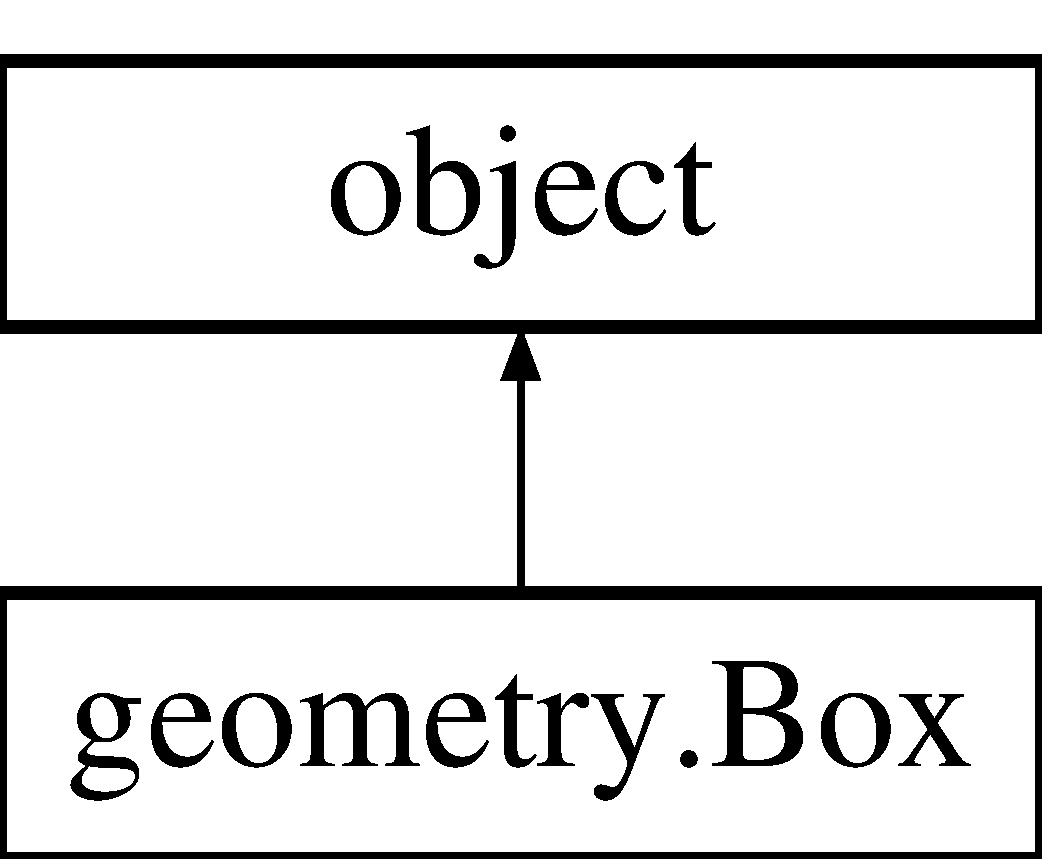
\includegraphics[height=2.000000cm]{classgeometry_1_1Box}
\end{center}
\end{figure}
\subsection*{Public Member Functions}
\begin{DoxyCompactItemize}
\item 
def \hyperlink{classgeometry_1_1Box_acd3c4e947c8bc7e6fe8efe8a05842238}{\+\_\+\+\_\+init\+\_\+\+\_\+} (self)
\item 
def \hyperlink{classgeometry_1_1Box_a9fed11ac430eeb493f1f9101ed50e570}{\+\_\+\+\_\+getitem\+\_\+\+\_\+} (self, ind)
\item 
def \hyperlink{classgeometry_1_1Box_afa830f6acc2fe66f4e9fb8a27921570f}{\+\_\+\+\_\+setitem\+\_\+\+\_\+} (self, ind, val)
\item 
\mbox{\Hypertarget{classgeometry_1_1Box_a8a830538d3a7a8e9022e55d3135d55a4}\label{classgeometry_1_1Box_a8a830538d3a7a8e9022e55d3135d55a4}} 
def {\bfseries \+\_\+\+\_\+str\+\_\+\+\_\+} (self)
\item 
def \hyperlink{classgeometry_1_1Box_ad6bd218082264a42a11c0d36ff3f8ff1}{\+\_\+\+\_\+cmp\+\_\+\+\_\+} (self, b)
\item 
def \hyperlink{classgeometry_1_1Box_a4b0f4675b22c67b531b00459cf6858b5}{add} (self, p)
\item 
def \hyperlink{classgeometry_1_1Box_af184892d7008637d2d34a9cc4fa4fdd5}{contains} (self, p)
\item 
def \hyperlink{classgeometry_1_1Box_af22304a33ca2c58b7ca21427608602e0}{contains2} (self, p)
\item 
def \hyperlink{classgeometry_1_1Box_aaab7456e78cc5b951e1b832b6816d332}{centre} (self)
\item 
def \hyperlink{classgeometry_1_1Box_af876b4d7ab7286682103a064e96f43d6}{len} (self)
\item 
def \hyperlink{classgeometry_1_1Box_a6bd75c486ba4bb587c3003484be1bc6d}{outside\+Position} (self)
\item 
def \hyperlink{classgeometry_1_1Box_a2af13fbaf9c38d904e05d73e35b5f9f9}{set\+Parameters} (self)
\item 
def \hyperlink{classgeometry_1_1Box_af671baed782da60af8058570b2f6bfa9}{normalize} (self, p)
\end{DoxyCompactItemize}
\subsection*{Public Attributes}
\begin{DoxyCompactItemize}
\item 
\hyperlink{classgeometry_1_1Box_aaa2928bad8272b83deb2cbe543b68c66}{ready}
\begin{DoxyCompactList}\small\item\em Set for lazy calculation of normalization parameters. \end{DoxyCompactList}\item 
\hyperlink{classgeometry_1_1Box_a6bf768dc4c7628cc2fe863eb3a002475}{bbox}
\begin{DoxyCompactList}\small\item\em A list with two points\+: the lower left corner and upper right corner of this box. \end{DoxyCompactList}\item 
\hyperlink{classgeometry_1_1Box_a43781b0f4c451cbb542c20b5fbd4b5dd}{sx}
\begin{DoxyCompactList}\small\item\em Scale factor x. \end{DoxyCompactList}\item 
\hyperlink{classgeometry_1_1Box_a0e744b5244823afefa01b40c2613037f}{tx}
\begin{DoxyCompactList}\small\item\em Translation factor x. \end{DoxyCompactList}\item 
\hyperlink{classgeometry_1_1Box_a223765001a3661705685ed85647a54ff}{sy}
\begin{DoxyCompactList}\small\item\em Scale factor y. \end{DoxyCompactList}\item 
\hyperlink{classgeometry_1_1Box_aca0410b99a6d8b59060f6fcbf12db160}{ty}
\begin{DoxyCompactList}\small\item\em Translation factor y. \end{DoxyCompactList}\end{DoxyCompactItemize}


\subsection{Detailed Description}
A bounging box is the smallest rectangle, aligned with the coordinate axes, which contain a given set of points. 

In CG, it can be used as an approximation for a geometric shape.\begin{DoxyVerb}A class for computing bounding boxes.\end{DoxyVerb}
 

Definition at line 581 of file geometry.\+py.



\subsection{Constructor \& Destructor Documentation}
\mbox{\Hypertarget{classgeometry_1_1Box_acd3c4e947c8bc7e6fe8efe8a05842238}\label{classgeometry_1_1Box_acd3c4e947c8bc7e6fe8efe8a05842238}} 
\index{geometry\+::\+Box@{geometry\+::\+Box}!\+\_\+\+\_\+init\+\_\+\+\_\+@{\+\_\+\+\_\+init\+\_\+\+\_\+}}
\index{\+\_\+\+\_\+init\+\_\+\+\_\+@{\+\_\+\+\_\+init\+\_\+\+\_\+}!geometry\+::\+Box@{geometry\+::\+Box}}
\subsubsection{\texorpdfstring{\+\_\+\+\_\+init\+\_\+\+\_\+()}{\_\_init\_\_()}}
{\footnotesize\ttfamily def geometry.\+Box.\+\_\+\+\_\+init\+\_\+\+\_\+ (\begin{DoxyParamCaption}\item[{}]{self }\end{DoxyParamCaption})}

\begin{DoxyVerb}Constructs an invalid bouding box.\end{DoxyVerb}
 

Definition at line 584 of file geometry.\+py.



\subsection{Member Function Documentation}
\mbox{\Hypertarget{classgeometry_1_1Box_ad6bd218082264a42a11c0d36ff3f8ff1}\label{classgeometry_1_1Box_ad6bd218082264a42a11c0d36ff3f8ff1}} 
\index{geometry\+::\+Box@{geometry\+::\+Box}!\+\_\+\+\_\+cmp\+\_\+\+\_\+@{\+\_\+\+\_\+cmp\+\_\+\+\_\+}}
\index{\+\_\+\+\_\+cmp\+\_\+\+\_\+@{\+\_\+\+\_\+cmp\+\_\+\+\_\+}!geometry\+::\+Box@{geometry\+::\+Box}}
\subsubsection{\texorpdfstring{\+\_\+\+\_\+cmp\+\_\+\+\_\+()}{\_\_cmp\_\_()}}
{\footnotesize\ttfamily def geometry.\+Box.\+\_\+\+\_\+cmp\+\_\+\+\_\+ (\begin{DoxyParamCaption}\item[{}]{self,  }\item[{}]{b }\end{DoxyParamCaption})}

\begin{DoxyVerb}Return < 0 if self < b, 
  > 0 if self > b,
    0 if self = b
\end{DoxyVerb}
 

Definition at line 605 of file geometry.\+py.

\mbox{\Hypertarget{classgeometry_1_1Box_a9fed11ac430eeb493f1f9101ed50e570}\label{classgeometry_1_1Box_a9fed11ac430eeb493f1f9101ed50e570}} 
\index{geometry\+::\+Box@{geometry\+::\+Box}!\+\_\+\+\_\+getitem\+\_\+\+\_\+@{\+\_\+\+\_\+getitem\+\_\+\+\_\+}}
\index{\+\_\+\+\_\+getitem\+\_\+\+\_\+@{\+\_\+\+\_\+getitem\+\_\+\+\_\+}!geometry\+::\+Box@{geometry\+::\+Box}}
\subsubsection{\texorpdfstring{\+\_\+\+\_\+getitem\+\_\+\+\_\+()}{\_\_getitem\_\_()}}
{\footnotesize\ttfamily def geometry.\+Box.\+\_\+\+\_\+getitem\+\_\+\+\_\+ (\begin{DoxyParamCaption}\item[{}]{self,  }\item[{}]{ind }\end{DoxyParamCaption})}

\begin{DoxyVerb}Indexing operator.\end{DoxyVerb}
 

Definition at line 592 of file geometry.\+py.

\mbox{\Hypertarget{classgeometry_1_1Box_afa830f6acc2fe66f4e9fb8a27921570f}\label{classgeometry_1_1Box_afa830f6acc2fe66f4e9fb8a27921570f}} 
\index{geometry\+::\+Box@{geometry\+::\+Box}!\+\_\+\+\_\+setitem\+\_\+\+\_\+@{\+\_\+\+\_\+setitem\+\_\+\+\_\+}}
\index{\+\_\+\+\_\+setitem\+\_\+\+\_\+@{\+\_\+\+\_\+setitem\+\_\+\+\_\+}!geometry\+::\+Box@{geometry\+::\+Box}}
\subsubsection{\texorpdfstring{\+\_\+\+\_\+setitem\+\_\+\+\_\+()}{\_\_setitem\_\_()}}
{\footnotesize\ttfamily def geometry.\+Box.\+\_\+\+\_\+setitem\+\_\+\+\_\+ (\begin{DoxyParamCaption}\item[{}]{self,  }\item[{}]{ind,  }\item[{}]{val }\end{DoxyParamCaption})}

\begin{DoxyVerb}Indexing operator.\end{DoxyVerb}
 

Definition at line 596 of file geometry.\+py.

\mbox{\Hypertarget{classgeometry_1_1Box_a4b0f4675b22c67b531b00459cf6858b5}\label{classgeometry_1_1Box_a4b0f4675b22c67b531b00459cf6858b5}} 
\index{geometry\+::\+Box@{geometry\+::\+Box}!add@{add}}
\index{add@{add}!geometry\+::\+Box@{geometry\+::\+Box}}
\subsubsection{\texorpdfstring{add()}{add()}}
{\footnotesize\ttfamily def geometry.\+Box.\+add (\begin{DoxyParamCaption}\item[{}]{self,  }\item[{}]{p }\end{DoxyParamCaption})}

\begin{DoxyVerb}Adds a new point to the bounding box.\end{DoxyVerb}
 

Definition at line 613 of file geometry.\+py.

\mbox{\Hypertarget{classgeometry_1_1Box_aaab7456e78cc5b951e1b832b6816d332}\label{classgeometry_1_1Box_aaab7456e78cc5b951e1b832b6816d332}} 
\index{geometry\+::\+Box@{geometry\+::\+Box}!centre@{centre}}
\index{centre@{centre}!geometry\+::\+Box@{geometry\+::\+Box}}
\subsubsection{\texorpdfstring{centre()}{centre()}}
{\footnotesize\ttfamily def geometry.\+Box.\+centre (\begin{DoxyParamCaption}\item[{}]{self }\end{DoxyParamCaption})}

\begin{DoxyVerb}Return the centre of the box.\end{DoxyVerb}
 

Definition at line 642 of file geometry.\+py.

\mbox{\Hypertarget{classgeometry_1_1Box_af184892d7008637d2d34a9cc4fa4fdd5}\label{classgeometry_1_1Box_af184892d7008637d2d34a9cc4fa4fdd5}} 
\index{geometry\+::\+Box@{geometry\+::\+Box}!contains@{contains}}
\index{contains@{contains}!geometry\+::\+Box@{geometry\+::\+Box}}
\subsubsection{\texorpdfstring{contains()}{contains()}}
{\footnotesize\ttfamily def geometry.\+Box.\+contains (\begin{DoxyParamCaption}\item[{}]{self,  }\item[{}]{p }\end{DoxyParamCaption})}

\begin{DoxyVerb}Return whether this box contains point p.\end{DoxyVerb}
 

Definition at line 629 of file geometry.\+py.

\mbox{\Hypertarget{classgeometry_1_1Box_af22304a33ca2c58b7ca21427608602e0}\label{classgeometry_1_1Box_af22304a33ca2c58b7ca21427608602e0}} 
\index{geometry\+::\+Box@{geometry\+::\+Box}!contains2@{contains2}}
\index{contains2@{contains2}!geometry\+::\+Box@{geometry\+::\+Box}}
\subsubsection{\texorpdfstring{contains2()}{contains2()}}
{\footnotesize\ttfamily def geometry.\+Box.\+contains2 (\begin{DoxyParamCaption}\item[{}]{self,  }\item[{}]{p }\end{DoxyParamCaption})}

\begin{DoxyVerb}Return whether this box contains point p.\end{DoxyVerb}
 

Definition at line 636 of file geometry.\+py.

\mbox{\Hypertarget{classgeometry_1_1Box_af876b4d7ab7286682103a064e96f43d6}\label{classgeometry_1_1Box_af876b4d7ab7286682103a064e96f43d6}} 
\index{geometry\+::\+Box@{geometry\+::\+Box}!len@{len}}
\index{len@{len}!geometry\+::\+Box@{geometry\+::\+Box}}
\subsubsection{\texorpdfstring{len()}{len()}}
{\footnotesize\ttfamily def geometry.\+Box.\+len (\begin{DoxyParamCaption}\item[{}]{self }\end{DoxyParamCaption})}

\begin{DoxyVerb}Return the length (a vector) of the box.\end{DoxyVerb}
 

Definition at line 646 of file geometry.\+py.

\mbox{\Hypertarget{classgeometry_1_1Box_af671baed782da60af8058570b2f6bfa9}\label{classgeometry_1_1Box_af671baed782da60af8058570b2f6bfa9}} 
\index{geometry\+::\+Box@{geometry\+::\+Box}!normalize@{normalize}}
\index{normalize@{normalize}!geometry\+::\+Box@{geometry\+::\+Box}}
\subsubsection{\texorpdfstring{normalize()}{normalize()}}
{\footnotesize\ttfamily def geometry.\+Box.\+normalize (\begin{DoxyParamCaption}\item[{}]{self,  }\item[{}]{p }\end{DoxyParamCaption})}

\begin{DoxyVerb}Normalize the given point.\end{DoxyVerb}
 

Definition at line 670 of file geometry.\+py.

\mbox{\Hypertarget{classgeometry_1_1Box_a6bd75c486ba4bb587c3003484be1bc6d}\label{classgeometry_1_1Box_a6bd75c486ba4bb587c3003484be1bc6d}} 
\index{geometry\+::\+Box@{geometry\+::\+Box}!outside\+Position@{outside\+Position}}
\index{outside\+Position@{outside\+Position}!geometry\+::\+Box@{geometry\+::\+Box}}
\subsubsection{\texorpdfstring{outside\+Position()}{outsidePosition()}}
{\footnotesize\ttfamily def geometry.\+Box.\+outside\+Position (\begin{DoxyParamCaption}\item[{}]{self }\end{DoxyParamCaption})}

\begin{DoxyVerb}Return a point outside the box.\end{DoxyVerb}
 

Definition at line 650 of file geometry.\+py.

\mbox{\Hypertarget{classgeometry_1_1Box_a2af13fbaf9c38d904e05d73e35b5f9f9}\label{classgeometry_1_1Box_a2af13fbaf9c38d904e05d73e35b5f9f9}} 
\index{geometry\+::\+Box@{geometry\+::\+Box}!set\+Parameters@{set\+Parameters}}
\index{set\+Parameters@{set\+Parameters}!geometry\+::\+Box@{geometry\+::\+Box}}
\subsubsection{\texorpdfstring{set\+Parameters()}{setParameters()}}
{\footnotesize\ttfamily def geometry.\+Box.\+set\+Parameters (\begin{DoxyParamCaption}\item[{}]{self }\end{DoxyParamCaption})}

\begin{DoxyVerb}Calculates the parameters to a normalized box.\end{DoxyVerb}
 

Definition at line 655 of file geometry.\+py.



\subsection{Member Data Documentation}
\mbox{\Hypertarget{classgeometry_1_1Box_a6bf768dc4c7628cc2fe863eb3a002475}\label{classgeometry_1_1Box_a6bf768dc4c7628cc2fe863eb3a002475}} 
\index{geometry\+::\+Box@{geometry\+::\+Box}!bbox@{bbox}}
\index{bbox@{bbox}!geometry\+::\+Box@{geometry\+::\+Box}}
\subsubsection{\texorpdfstring{bbox}{bbox}}
{\footnotesize\ttfamily geometry.\+Box.\+bbox}



A list with two points\+: the lower left corner and upper right corner of this box. 



Definition at line 590 of file geometry.\+py.

\mbox{\Hypertarget{classgeometry_1_1Box_aaa2928bad8272b83deb2cbe543b68c66}\label{classgeometry_1_1Box_aaa2928bad8272b83deb2cbe543b68c66}} 
\index{geometry\+::\+Box@{geometry\+::\+Box}!ready@{ready}}
\index{ready@{ready}!geometry\+::\+Box@{geometry\+::\+Box}}
\subsubsection{\texorpdfstring{ready}{ready}}
{\footnotesize\ttfamily geometry.\+Box.\+ready}



Set for lazy calculation of normalization parameters. 



Definition at line 588 of file geometry.\+py.

\mbox{\Hypertarget{classgeometry_1_1Box_a43781b0f4c451cbb542c20b5fbd4b5dd}\label{classgeometry_1_1Box_a43781b0f4c451cbb542c20b5fbd4b5dd}} 
\index{geometry\+::\+Box@{geometry\+::\+Box}!sx@{sx}}
\index{sx@{sx}!geometry\+::\+Box@{geometry\+::\+Box}}
\subsubsection{\texorpdfstring{sx}{sx}}
{\footnotesize\ttfamily geometry.\+Box.\+sx}



Scale factor x. 



Definition at line 659 of file geometry.\+py.

\mbox{\Hypertarget{classgeometry_1_1Box_a223765001a3661705685ed85647a54ff}\label{classgeometry_1_1Box_a223765001a3661705685ed85647a54ff}} 
\index{geometry\+::\+Box@{geometry\+::\+Box}!sy@{sy}}
\index{sy@{sy}!geometry\+::\+Box@{geometry\+::\+Box}}
\subsubsection{\texorpdfstring{sy}{sy}}
{\footnotesize\ttfamily geometry.\+Box.\+sy}



Scale factor y. 



Definition at line 664 of file geometry.\+py.

\mbox{\Hypertarget{classgeometry_1_1Box_a0e744b5244823afefa01b40c2613037f}\label{classgeometry_1_1Box_a0e744b5244823afefa01b40c2613037f}} 
\index{geometry\+::\+Box@{geometry\+::\+Box}!tx@{tx}}
\index{tx@{tx}!geometry\+::\+Box@{geometry\+::\+Box}}
\subsubsection{\texorpdfstring{tx}{tx}}
{\footnotesize\ttfamily geometry.\+Box.\+tx}



Translation factor x. 



Definition at line 661 of file geometry.\+py.

\mbox{\Hypertarget{classgeometry_1_1Box_aca0410b99a6d8b59060f6fcbf12db160}\label{classgeometry_1_1Box_aca0410b99a6d8b59060f6fcbf12db160}} 
\index{geometry\+::\+Box@{geometry\+::\+Box}!ty@{ty}}
\index{ty@{ty}!geometry\+::\+Box@{geometry\+::\+Box}}
\subsubsection{\texorpdfstring{ty}{ty}}
{\footnotesize\ttfamily geometry.\+Box.\+ty}



Translation factor y. 



Definition at line 666 of file geometry.\+py.



The documentation for this class was generated from the following file\+:\begin{DoxyCompactItemize}
\item 
geometry.\+py\end{DoxyCompactItemize}

\hypertarget{classadditional__classes_1_1ColoredPolygon}{}\section{additional\+\_\+classes.\+Colored\+Polygon Class Reference}
\label{classadditional__classes_1_1ColoredPolygon}\index{additional\+\_\+classes.\+Colored\+Polygon@{additional\+\_\+classes.\+Colored\+Polygon}}


Class that extends the Polygon class from the geometry module.  


Inheritance diagram for additional\+\_\+classes.\+Colored\+Polygon\+:\begin{figure}[H]
\begin{center}
\leavevmode
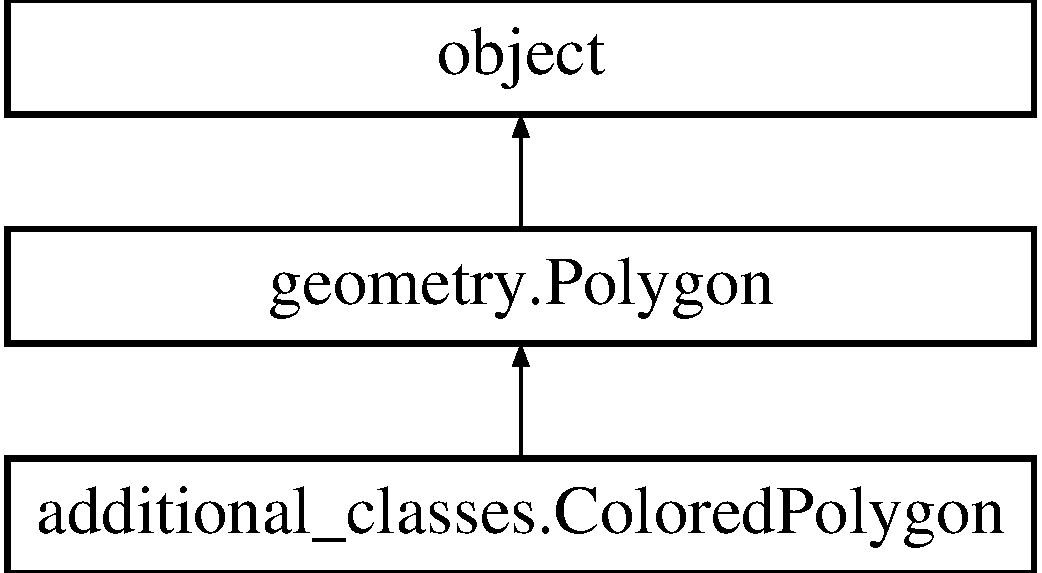
\includegraphics[height=3.000000cm]{classadditional__classes_1_1ColoredPolygon}
\end{center}
\end{figure}
\subsection*{Public Member Functions}
\begin{DoxyCompactItemize}
\item 
\mbox{\Hypertarget{classadditional__classes_1_1ColoredPolygon_a4500b4e5c51f3a99d80042378c3ccc7a}\label{classadditional__classes_1_1ColoredPolygon_a4500b4e5c51f3a99d80042378c3ccc7a}} 
def \hyperlink{classadditional__classes_1_1ColoredPolygon_a4500b4e5c51f3a99d80042378c3ccc7a}{\+\_\+\+\_\+init\+\_\+\+\_\+} (self, \hyperlink{classgeometry_1_1Polygon_aa0fda1ff74a09b8498bd7d8731b2fbf1}{points}, r, g, b)
\begin{DoxyCompactList}\small\item\em The constructor. \end{DoxyCompactList}\item 
def \hyperlink{classadditional__classes_1_1ColoredPolygon_a8c7c8ef66ef3bfddc0223c109addab48}{set\+Color} (self, r, g, b)
\begin{DoxyCompactList}\small\item\em Sets the polygon color. \end{DoxyCompactList}\item 
def \hyperlink{classadditional__classes_1_1ColoredPolygon_a3ba3e35b383cc6999480057a4d026e71}{center\+Point} (self)
\begin{DoxyCompactList}\small\item\em Defines the center point of the polygon using a bounding box. \end{DoxyCompactList}\end{DoxyCompactItemize}
\subsection*{Public Attributes}
\begin{DoxyCompactItemize}
\item 
\mbox{\Hypertarget{classadditional__classes_1_1ColoredPolygon_a295d9e1070e4d575743c49de93445682}\label{classadditional__classes_1_1ColoredPolygon_a295d9e1070e4d575743c49de93445682}} 
{\bfseries r}
\item 
\mbox{\Hypertarget{classadditional__classes_1_1ColoredPolygon_ac2746b0396a46ec9effcc8f90d565e71}\label{classadditional__classes_1_1ColoredPolygon_ac2746b0396a46ec9effcc8f90d565e71}} 
{\bfseries g}
\item 
\mbox{\Hypertarget{classadditional__classes_1_1ColoredPolygon_aba7d007dc6febd0340a7097f7aca3cc4}\label{classadditional__classes_1_1ColoredPolygon_aba7d007dc6febd0340a7097f7aca3cc4}} 
{\bfseries b}
\item 
\mbox{\Hypertarget{classadditional__classes_1_1ColoredPolygon_ae98eb7632de780c284f816bbe61048f0}\label{classadditional__classes_1_1ColoredPolygon_ae98eb7632de780c284f816bbe61048f0}} 
{\bfseries parents}
\item 
\mbox{\Hypertarget{classadditional__classes_1_1ColoredPolygon_ae3cfb699daba9fbf0ecb216844e0c62b}\label{classadditional__classes_1_1ColoredPolygon_ae3cfb699daba9fbf0ecb216844e0c62b}} 
{\bfseries children}
\item 
\mbox{\Hypertarget{classadditional__classes_1_1ColoredPolygon_a2a6a05cb4c03964b8a6ca44aa5fe286d}\label{classadditional__classes_1_1ColoredPolygon_a2a6a05cb4c03964b8a6ca44aa5fe286d}} 
{\bfseries nails}
\end{DoxyCompactItemize}


\subsection{Detailed Description}
Class that extends the Polygon class from the geometry module. 

Added color and the data structures necessary to implement the transformation hierarchy. 

Definition at line 12 of file additional\+\_\+classes.\+py.



\subsection{Member Function Documentation}
\mbox{\Hypertarget{classadditional__classes_1_1ColoredPolygon_a3ba3e35b383cc6999480057a4d026e71}\label{classadditional__classes_1_1ColoredPolygon_a3ba3e35b383cc6999480057a4d026e71}} 
\index{additional\+\_\+classes\+::\+Colored\+Polygon@{additional\+\_\+classes\+::\+Colored\+Polygon}!center\+Point@{center\+Point}}
\index{center\+Point@{center\+Point}!additional\+\_\+classes\+::\+Colored\+Polygon@{additional\+\_\+classes\+::\+Colored\+Polygon}}
\subsubsection{\texorpdfstring{center\+Point()}{centerPoint()}}
{\footnotesize\ttfamily def additional\+\_\+classes.\+Colored\+Polygon.\+center\+Point (\begin{DoxyParamCaption}\item[{}]{self }\end{DoxyParamCaption})}



Defines the center point of the polygon using a bounding box. 


\begin{DoxyParams}{Parameters}
{\em self} & The \hyperlink{classadditional__classes_1_1ColoredPolygon}{Colored\+Polygon} object \\
\hline
\end{DoxyParams}
\begin{DoxyReturn}{Returns}
Returns the center of the polygon 
\end{DoxyReturn}


Definition at line 37 of file additional\+\_\+classes.\+py.

\mbox{\Hypertarget{classadditional__classes_1_1ColoredPolygon_a8c7c8ef66ef3bfddc0223c109addab48}\label{classadditional__classes_1_1ColoredPolygon_a8c7c8ef66ef3bfddc0223c109addab48}} 
\index{additional\+\_\+classes\+::\+Colored\+Polygon@{additional\+\_\+classes\+::\+Colored\+Polygon}!set\+Color@{set\+Color}}
\index{set\+Color@{set\+Color}!additional\+\_\+classes\+::\+Colored\+Polygon@{additional\+\_\+classes\+::\+Colored\+Polygon}}
\subsubsection{\texorpdfstring{set\+Color()}{setColor()}}
{\footnotesize\ttfamily def additional\+\_\+classes.\+Colored\+Polygon.\+set\+Color (\begin{DoxyParamCaption}\item[{}]{self,  }\item[{}]{r,  }\item[{}]{g,  }\item[{}]{b }\end{DoxyParamCaption})}



Sets the polygon color. 


\begin{DoxyParams}{Parameters}
{\em self} & The \hyperlink{classadditional__classes_1_1ColoredPolygon}{Colored\+Polygon} object \\
\hline
{\em r} & The red parameter of R\+GB \\
\hline
{\em g} & The green parameter of R\+GB \\
\hline
{\em b} & The blue parameter of R\+GB \\
\hline
\end{DoxyParams}


Definition at line 29 of file additional\+\_\+classes.\+py.



The documentation for this class was generated from the following file\+:\begin{DoxyCompactItemize}
\item 
additional\+\_\+classes.\+py\end{DoxyCompactItemize}

\hypertarget{classadditional__classes_1_1DoubleClick}{}\section{additional\+\_\+classes.\+Double\+Click Class Reference}
\label{classadditional__classes_1_1DoubleClick}\index{additional\+\_\+classes.\+Double\+Click@{additional\+\_\+classes.\+Double\+Click}}


Class that implements the double click logic, used to place the nails.  


Inheritance diagram for additional\+\_\+classes.\+Double\+Click\+:\begin{figure}[H]
\begin{center}
\leavevmode
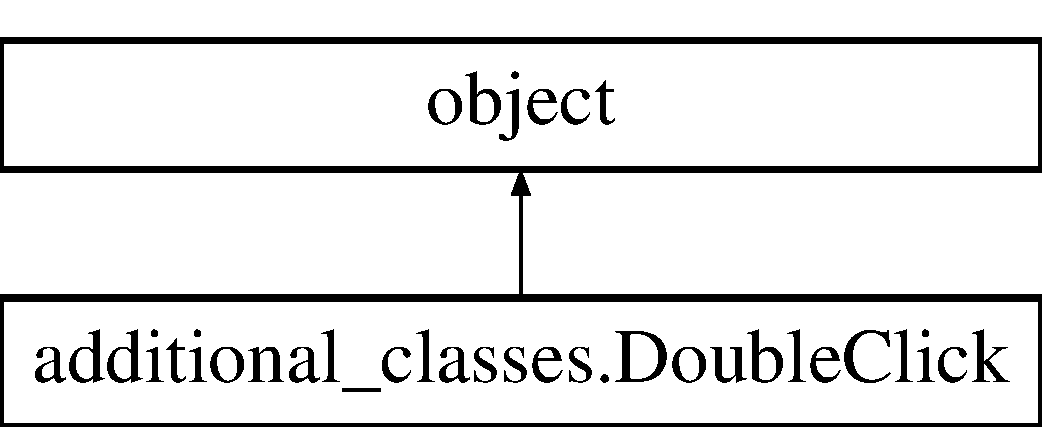
\includegraphics[height=2.000000cm]{classadditional__classes_1_1DoubleClick}
\end{center}
\end{figure}
\subsection*{Public Member Functions}
\begin{DoxyCompactItemize}
\item 
\mbox{\Hypertarget{classadditional__classes_1_1DoubleClick_aeda7ebb4d2db48777c252d470eeb180e}\label{classadditional__classes_1_1DoubleClick_aeda7ebb4d2db48777c252d470eeb180e}} 
def \hyperlink{classadditional__classes_1_1DoubleClick_aeda7ebb4d2db48777c252d470eeb180e}{\+\_\+\+\_\+init\+\_\+\+\_\+} (self, time)
\begin{DoxyCompactList}\small\item\em The constructor. \end{DoxyCompactList}\item 
\mbox{\Hypertarget{classadditional__classes_1_1DoubleClick_a428626cbc162531871957a35bcaa8b19}\label{classadditional__classes_1_1DoubleClick_a428626cbc162531871957a35bcaa8b19}} 
def \hyperlink{classadditional__classes_1_1DoubleClick_a428626cbc162531871957a35bcaa8b19}{is\+Double\+Clicked} (self, final\+Time)
\begin{DoxyCompactList}\small\item\em Checks if the clicks are single or double clicks. \end{DoxyCompactList}\end{DoxyCompactItemize}
\subsection*{Public Attributes}
\begin{DoxyCompactItemize}
\item 
\mbox{\Hypertarget{classadditional__classes_1_1DoubleClick_aeaecde73ab3539246d00807f727e03be}\label{classadditional__classes_1_1DoubleClick_aeaecde73ab3539246d00807f727e03be}} 
{\bfseries time}
\end{DoxyCompactItemize}


\subsection{Detailed Description}
Class that implements the double click logic, used to place the nails. 

Definition at line 45 of file additional\+\_\+classes.\+py.



The documentation for this class was generated from the following file\+:\begin{DoxyCompactItemize}
\item 
additional\+\_\+classes.\+py\end{DoxyCompactItemize}

\hypertarget{classgeometry_1_1Line}{}\section{geometry.\+Line Class Reference}
\label{classgeometry_1_1Line}\index{geometry.\+Line@{geometry.\+Line}}


Two points define a straight line.  


Inheritance diagram for geometry.\+Line\+:\begin{figure}[H]
\begin{center}
\leavevmode
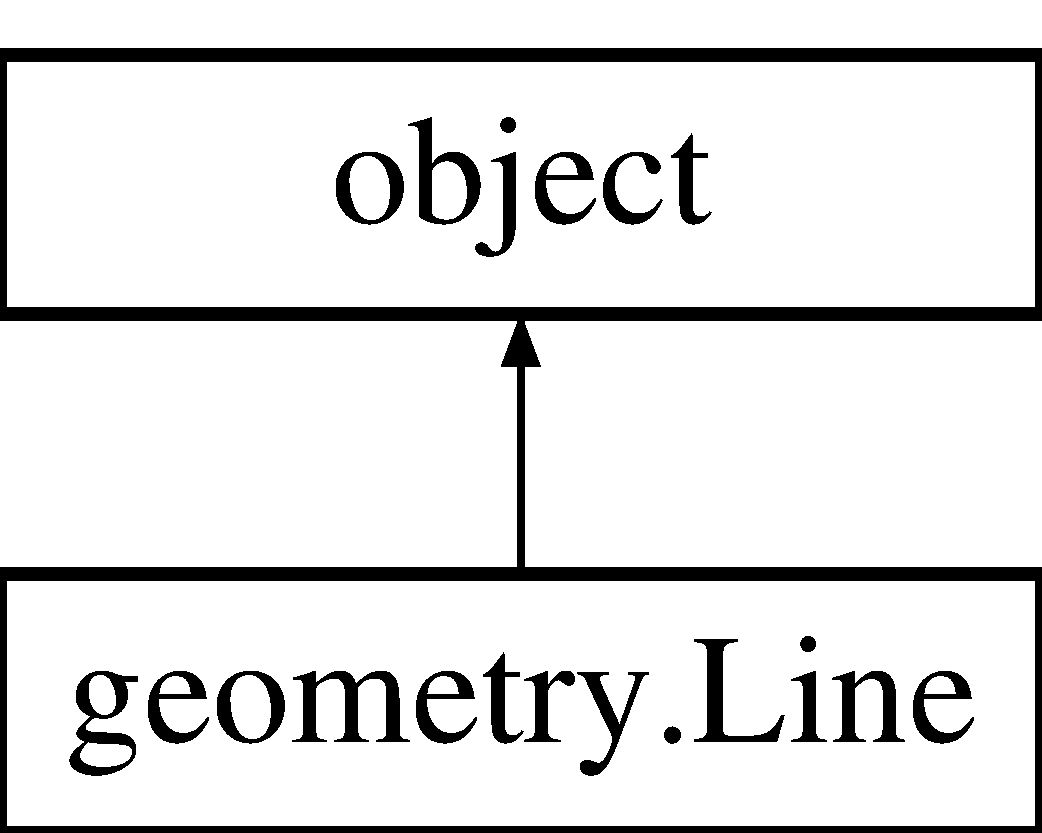
\includegraphics[height=2.000000cm]{classgeometry_1_1Line}
\end{center}
\end{figure}
\subsection*{Public Member Functions}
\begin{DoxyCompactItemize}
\item 
\mbox{\Hypertarget{classgeometry_1_1Line_a0798ab42b8ca969cc6b686085642e023}\label{classgeometry_1_1Line_a0798ab42b8ca969cc6b686085642e023}} 
def {\bfseries \+\_\+\+\_\+init\+\_\+\+\_\+} (self, \hyperlink{classgeometry_1_1Line_aa46ea22a1b33099cbfa26a1646595a40}{p1}, \hyperlink{classgeometry_1_1Line_a10b5fbbd99ed5d63848a09e50a782cdf}{p2})
\item 
\mbox{\Hypertarget{classgeometry_1_1Line_ac5887251dccbea9ec1fbab00dcfc42aa}\label{classgeometry_1_1Line_ac5887251dccbea9ec1fbab00dcfc42aa}} 
def {\bfseries \+\_\+\+\_\+repr\+\_\+\+\_\+} (self)
\item 
\mbox{\Hypertarget{classgeometry_1_1Line_a0b21cc539996c6afb8f0fc1763d9d174}\label{classgeometry_1_1Line_a0b21cc539996c6afb8f0fc1763d9d174}} 
def {\bfseries \+\_\+\+\_\+eq\+\_\+\+\_\+} (self, other)
\item 
def \hyperlink{classgeometry_1_1Line_a05b2f8b25c0025ba627523dc137f66cb}{atT} (self, t)
\item 
def \hyperlink{classgeometry_1_1Line_ac6b10e2377ad195ca3c2a6148b1aa770}{distance} (self, p)
\end{DoxyCompactItemize}
\subsection*{Public Attributes}
\begin{DoxyCompactItemize}
\item 
\mbox{\Hypertarget{classgeometry_1_1Line_aa46ea22a1b33099cbfa26a1646595a40}\label{classgeometry_1_1Line_aa46ea22a1b33099cbfa26a1646595a40}} 
\hyperlink{classgeometry_1_1Line_aa46ea22a1b33099cbfa26a1646595a40}{p1}
\begin{DoxyCompactList}\small\item\em line starting point \end{DoxyCompactList}\item 
\mbox{\Hypertarget{classgeometry_1_1Line_a10b5fbbd99ed5d63848a09e50a782cdf}\label{classgeometry_1_1Line_a10b5fbbd99ed5d63848a09e50a782cdf}} 
\hyperlink{classgeometry_1_1Line_a10b5fbbd99ed5d63848a09e50a782cdf}{p2}
\begin{DoxyCompactList}\small\item\em line ending point \end{DoxyCompactList}\item 
\mbox{\Hypertarget{classgeometry_1_1Line_a184c36a24c5e66becce19c0fe53c8b95}\label{classgeometry_1_1Line_a184c36a24c5e66becce19c0fe53c8b95}} 
\hyperlink{classgeometry_1_1Line_a184c36a24c5e66becce19c0fe53c8b95}{dir}
\begin{DoxyCompactList}\small\item\em line direction \end{DoxyCompactList}\end{DoxyCompactItemize}


\subsection{Detailed Description}
Two points define a straight line. 

A line is represented by a starting (or origin) and ending points, thus defining a direction.\begin{DoxyVerb}A class representing a line.\end{DoxyVerb}
 

Definition at line 212 of file geometry.\+py.



\subsection{Member Function Documentation}
\mbox{\Hypertarget{classgeometry_1_1Line_a05b2f8b25c0025ba627523dc137f66cb}\label{classgeometry_1_1Line_a05b2f8b25c0025ba627523dc137f66cb}} 
\index{geometry\+::\+Line@{geometry\+::\+Line}!atT@{atT}}
\index{atT@{atT}!geometry\+::\+Line@{geometry\+::\+Line}}
\subsubsection{\texorpdfstring{at\+T()}{atT()}}
{\footnotesize\ttfamily def geometry.\+Line.\+atT (\begin{DoxyParamCaption}\item[{}]{self,  }\item[{}]{t }\end{DoxyParamCaption})}

\begin{DoxyVerb}Evaluates this line at parameter t.\end{DoxyVerb}
 

Definition at line 232 of file geometry.\+py.

\mbox{\Hypertarget{classgeometry_1_1Line_ac6b10e2377ad195ca3c2a6148b1aa770}\label{classgeometry_1_1Line_ac6b10e2377ad195ca3c2a6148b1aa770}} 
\index{geometry\+::\+Line@{geometry\+::\+Line}!distance@{distance}}
\index{distance@{distance}!geometry\+::\+Line@{geometry\+::\+Line}}
\subsubsection{\texorpdfstring{distance()}{distance()}}
{\footnotesize\ttfamily def geometry.\+Line.\+distance (\begin{DoxyParamCaption}\item[{}]{self,  }\item[{}]{p }\end{DoxyParamCaption})}

\begin{DoxyVerb}Computes the distance from this line to a given point.

   @see http://mathworld.wolfram.com/Point-LineDistance3-Dimensional.html
\end{DoxyVerb}
 

Definition at line 237 of file geometry.\+py.



The documentation for this class was generated from the following file\+:\begin{DoxyCompactItemize}
\item 
geometry.\+py\end{DoxyCompactItemize}

\hypertarget{classgeometry_1_1Point}{}\section{geometry.\+Point Class Reference}
\label{classgeometry_1_1Point}\index{geometry.\+Point@{geometry.\+Point}}


Implements a 3D point or vector.  


Inheritance diagram for geometry.\+Point\+:\begin{figure}[H]
\begin{center}
\leavevmode
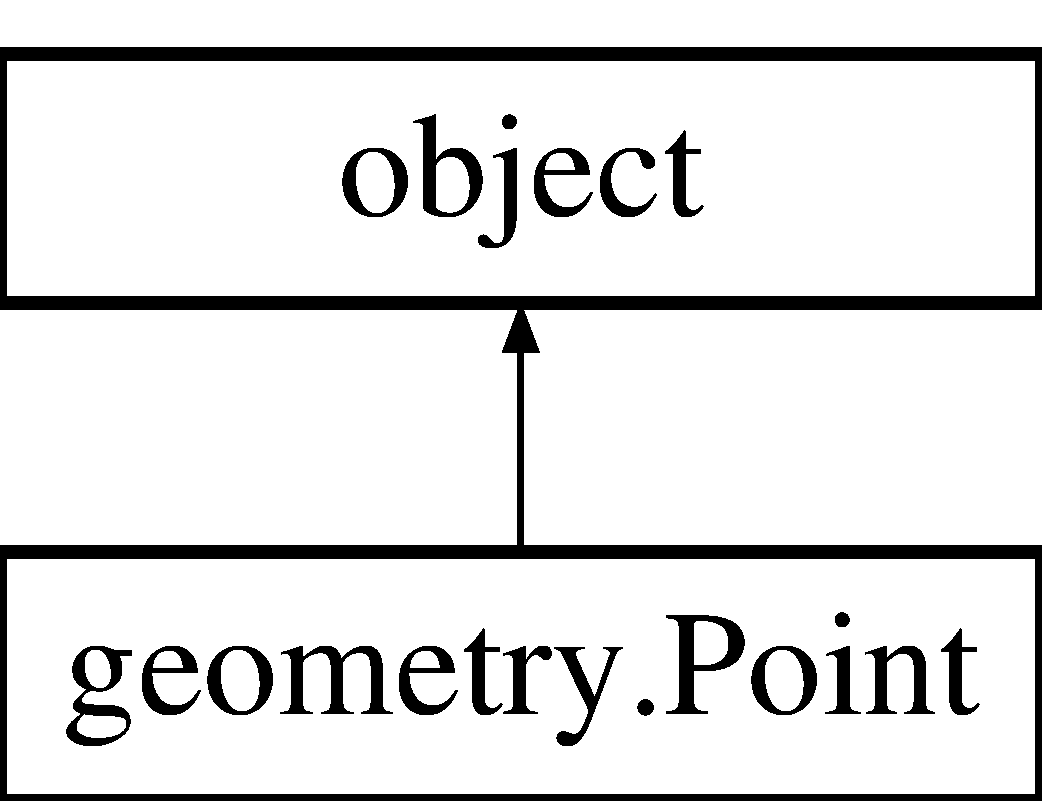
\includegraphics[height=2.000000cm]{classgeometry_1_1Point}
\end{center}
\end{figure}
\subsection*{Public Member Functions}
\begin{DoxyCompactItemize}
\item 
def \hyperlink{classgeometry_1_1Point_accb3af71f20d5531f1a478c4f5ca8105}{\+\_\+\+\_\+init\+\_\+\+\_\+} (self, \hyperlink{classgeometry_1_1Point_a98f21eef44d1c182f04f1262c90815fc}{x}, \hyperlink{classgeometry_1_1Point_a4ef9a436e11219296ba5e3fff9e87711}{y}, \hyperlink{classgeometry_1_1Point_afd1ce6427fa3e28c9c42934bb5d76165}{z}=0.\+0)
\begin{DoxyCompactList}\small\item\em \hyperlink{classgeometry_1_1Point}{Point} constructor. \end{DoxyCompactList}\item 
def \hyperlink{classgeometry_1_1Point_aebe045ef26f241b525459dfa1ee3b85f}{\+\_\+\+\_\+repr\+\_\+\+\_\+} (self)
\begin{DoxyCompactList}\small\item\em Print object. \end{DoxyCompactList}\item 
\mbox{\Hypertarget{classgeometry_1_1Point_a9cbf68fff40fffb87e6acff640c95294}\label{classgeometry_1_1Point_a9cbf68fff40fffb87e6acff640c95294}} 
def \hyperlink{classgeometry_1_1Point_a9cbf68fff40fffb87e6acff640c95294}{\+\_\+\+\_\+eq\+\_\+\+\_\+} (self, other)
\begin{DoxyCompactList}\small\item\em Operator ==. \end{DoxyCompactList}\item 
def \hyperlink{classgeometry_1_1Point_ae9e26dfa297c49feb6e0c2808c74bba8}{\+\_\+\+\_\+hash\+\_\+\+\_\+} (self)
\begin{DoxyCompactList}\small\item\em Should return the same value for objects that are equal. \end{DoxyCompactList}\item 
def \hyperlink{classgeometry_1_1Point_a68cd5b720a72a8c546c2b11b60d2dd76}{\+\_\+\+\_\+getitem\+\_\+\+\_\+} (self, ind)
\begin{DoxyCompactList}\small\item\em Indexing operator. \end{DoxyCompactList}\item 
def \hyperlink{classgeometry_1_1Point_aae8560cc5718faf25f3cb70942a32395}{\+\_\+\+\_\+setitem\+\_\+\+\_\+} (self, ind, val)
\begin{DoxyCompactList}\small\item\em Indexing operator. \end{DoxyCompactList}\item 
\mbox{\Hypertarget{classgeometry_1_1Point_a9ada2b2ca2dbc3dc42665fd218bc4244}\label{classgeometry_1_1Point_a9ada2b2ca2dbc3dc42665fd218bc4244}} 
def \hyperlink{classgeometry_1_1Point_a9ada2b2ca2dbc3dc42665fd218bc4244}{\+\_\+\+\_\+add\+\_\+\+\_\+} (self, other)
\begin{DoxyCompactList}\small\item\em Operator +. \end{DoxyCompactList}\item 
\mbox{\Hypertarget{classgeometry_1_1Point_a141cda9317590cdc109610b17a07249f}\label{classgeometry_1_1Point_a141cda9317590cdc109610b17a07249f}} 
def \hyperlink{classgeometry_1_1Point_a141cda9317590cdc109610b17a07249f}{\+\_\+\+\_\+neg\+\_\+\+\_\+} (self)
\begin{DoxyCompactList}\small\item\em Operator negation (-\/self) \end{DoxyCompactList}\item 
\mbox{\Hypertarget{classgeometry_1_1Point_ae2be6f6c6a6d6a43355225ab26533dad}\label{classgeometry_1_1Point_ae2be6f6c6a6d6a43355225ab26533dad}} 
def \hyperlink{classgeometry_1_1Point_ae2be6f6c6a6d6a43355225ab26533dad}{\+\_\+\+\_\+sub\+\_\+\+\_\+} (self, other)
\begin{DoxyCompactList}\small\item\em Operator -\/. \end{DoxyCompactList}\item 
\mbox{\Hypertarget{classgeometry_1_1Point_a2bc744353849f1680e960ee5092d1ac4}\label{classgeometry_1_1Point_a2bc744353849f1680e960ee5092d1ac4}} 
def \hyperlink{classgeometry_1_1Point_a2bc744353849f1680e960ee5092d1ac4}{\+\_\+\+\_\+rmul\+\_\+\+\_\+} (self, c)
\begin{DoxyCompactList}\small\item\em Operator self $\ast$ c. \end{DoxyCompactList}\item 
\mbox{\Hypertarget{classgeometry_1_1Point_a6e7eb112430d791c348f970ee0b133cc}\label{classgeometry_1_1Point_a6e7eb112430d791c348f970ee0b133cc}} 
def \hyperlink{classgeometry_1_1Point_a6e7eb112430d791c348f970ee0b133cc}{\+\_\+\+\_\+lmul\+\_\+\+\_\+} (self, c)
\begin{DoxyCompactList}\small\item\em Operator c $\ast$ self. \end{DoxyCompactList}\item 
\mbox{\Hypertarget{classgeometry_1_1Point_a07650758ee8b4493ac73042817e98aa5}\label{classgeometry_1_1Point_a07650758ee8b4493ac73042817e98aa5}} 
def \hyperlink{classgeometry_1_1Point_a07650758ee8b4493ac73042817e98aa5}{\+\_\+\+\_\+imul\+\_\+\+\_\+} (self, c)
\begin{DoxyCompactList}\small\item\em Operator $\ast$=. \end{DoxyCompactList}\item 
def \hyperlink{classgeometry_1_1Point_ab9ec6d1fd080ba8b7eb99e5832505c85}{close} (self, that, epsilon=\hyperlink{namespacegeometry_a543db87a5e9af9e1d17146559a540276}{E\+PS})
\item 
def \hyperlink{classgeometry_1_1Point_a8da689422b3b004369e1467f8123e8a7}{dist} (self, that)
\item 
def \hyperlink{classgeometry_1_1Point_a28f393df5b0c4a297157a3ae55f1f4a3}{sqr\+Dist} (self, that)
\item 
def \hyperlink{classgeometry_1_1Point_a12ce9dea666d1b40218822a89bada540}{np3} (self)
\item 
def \hyperlink{classgeometry_1_1Point_a133d82361f16f975fcb232ba41ff5562}{np} (self)
\item 
def \hyperlink{classgeometry_1_1Point_a4df6e13ff003843f967090fb7f51cc85}{dot\+Prod} (self, vec)
\item 
def \hyperlink{classgeometry_1_1Point_ae6747fdae2c6ec09961298171862ef4b}{cross\+Prod2d} (self, vec)
\item 
def \hyperlink{classgeometry_1_1Point_aa9a3448e0da24f3132a4ccc7abf191a7}{cross\+Prod} (self, vec)
\item 
def \hyperlink{classgeometry_1_1Point_acce6c690969f757d26e4a544955cb8f4}{triple\+Prod} (self, vec0, vec1)
\item 
def \hyperlink{classgeometry_1_1Point_ae6b226778d9c084c9369faa6dfd95398}{len} (self)
\item 
\mbox{\Hypertarget{classgeometry_1_1Point_a902f60cc3736617d3846e137a1efef80}\label{classgeometry_1_1Point_a902f60cc3736617d3846e137a1efef80}} 
def {\bfseries normalize} (self)
\end{DoxyCompactItemize}
\subsection*{Public Attributes}
\begin{DoxyCompactItemize}
\item 
\mbox{\Hypertarget{classgeometry_1_1Point_a98f21eef44d1c182f04f1262c90815fc}\label{classgeometry_1_1Point_a98f21eef44d1c182f04f1262c90815fc}} 
\hyperlink{classgeometry_1_1Point_a98f21eef44d1c182f04f1262c90815fc}{x}
\begin{DoxyCompactList}\small\item\em X coordinate. \end{DoxyCompactList}\item 
\mbox{\Hypertarget{classgeometry_1_1Point_a4ef9a436e11219296ba5e3fff9e87711}\label{classgeometry_1_1Point_a4ef9a436e11219296ba5e3fff9e87711}} 
\hyperlink{classgeometry_1_1Point_a4ef9a436e11219296ba5e3fff9e87711}{y}
\begin{DoxyCompactList}\small\item\em Y coordinate. \end{DoxyCompactList}\item 
\mbox{\Hypertarget{classgeometry_1_1Point_afd1ce6427fa3e28c9c42934bb5d76165}\label{classgeometry_1_1Point_afd1ce6427fa3e28c9c42934bb5d76165}} 
\hyperlink{classgeometry_1_1Point_afd1ce6427fa3e28c9c42934bb5d76165}{z}
\begin{DoxyCompactList}\small\item\em Z coordinate. \end{DoxyCompactList}\end{DoxyCompactItemize}


\subsection{Detailed Description}
Implements a 3D point or vector. 

Points are locations in space. Vectors are displacements in space.

A point in n-\/dimensional space is given by an n-\/tuple P=(p1,p2,...pn), where each coordinate pi is a scalar number.

A vector represents magnitude and direction in space, and is given by an n-\/tuple v=(v1,v2,...vn)=(vi), where each coordinate vi is a scalar.


\begin{DoxyItemize}
\item vector + vector = vector.
\item vector -\/ vector = vector.
\item point + vector = point.
\item point -\/ point = vector.
\item point + point is undefined.\begin{DoxyVerb}A class representing a point or a vector.\end{DoxyVerb}
 
\end{DoxyItemize}

Definition at line 55 of file geometry.\+py.



\subsection{Constructor \& Destructor Documentation}
\mbox{\Hypertarget{classgeometry_1_1Point_accb3af71f20d5531f1a478c4f5ca8105}\label{classgeometry_1_1Point_accb3af71f20d5531f1a478c4f5ca8105}} 
\index{geometry\+::\+Point@{geometry\+::\+Point}!\+\_\+\+\_\+init\+\_\+\+\_\+@{\+\_\+\+\_\+init\+\_\+\+\_\+}}
\index{\+\_\+\+\_\+init\+\_\+\+\_\+@{\+\_\+\+\_\+init\+\_\+\+\_\+}!geometry\+::\+Point@{geometry\+::\+Point}}
\subsubsection{\texorpdfstring{\+\_\+\+\_\+init\+\_\+\+\_\+()}{\_\_init\_\_()}}
{\footnotesize\ttfamily def geometry.\+Point.\+\_\+\+\_\+init\+\_\+\+\_\+ (\begin{DoxyParamCaption}\item[{}]{self,  }\item[{}]{x,  }\item[{}]{y,  }\item[{}]{z = {\ttfamily 0.0} }\end{DoxyParamCaption})}



\hyperlink{classgeometry_1_1Point}{Point} constructor. 



Definition at line 59 of file geometry.\+py.



\subsection{Member Function Documentation}
\mbox{\Hypertarget{classgeometry_1_1Point_a68cd5b720a72a8c546c2b11b60d2dd76}\label{classgeometry_1_1Point_a68cd5b720a72a8c546c2b11b60d2dd76}} 
\index{geometry\+::\+Point@{geometry\+::\+Point}!\+\_\+\+\_\+getitem\+\_\+\+\_\+@{\+\_\+\+\_\+getitem\+\_\+\+\_\+}}
\index{\+\_\+\+\_\+getitem\+\_\+\+\_\+@{\+\_\+\+\_\+getitem\+\_\+\+\_\+}!geometry\+::\+Point@{geometry\+::\+Point}}
\subsubsection{\texorpdfstring{\+\_\+\+\_\+getitem\+\_\+\+\_\+()}{\_\_getitem\_\_()}}
{\footnotesize\ttfamily def geometry.\+Point.\+\_\+\+\_\+getitem\+\_\+\+\_\+ (\begin{DoxyParamCaption}\item[{}]{self,  }\item[{}]{ind }\end{DoxyParamCaption})}



Indexing operator. 



Definition at line 85 of file geometry.\+py.

\mbox{\Hypertarget{classgeometry_1_1Point_ae9e26dfa297c49feb6e0c2808c74bba8}\label{classgeometry_1_1Point_ae9e26dfa297c49feb6e0c2808c74bba8}} 
\index{geometry\+::\+Point@{geometry\+::\+Point}!\+\_\+\+\_\+hash\+\_\+\+\_\+@{\+\_\+\+\_\+hash\+\_\+\+\_\+}}
\index{\+\_\+\+\_\+hash\+\_\+\+\_\+@{\+\_\+\+\_\+hash\+\_\+\+\_\+}!geometry\+::\+Point@{geometry\+::\+Point}}
\subsubsection{\texorpdfstring{\+\_\+\+\_\+hash\+\_\+\+\_\+()}{\_\_hash\_\_()}}
{\footnotesize\ttfamily def geometry.\+Point.\+\_\+\+\_\+hash\+\_\+\+\_\+ (\begin{DoxyParamCaption}\item[{}]{self }\end{DoxyParamCaption})}



Should return the same value for objects that are equal. 

It also shouldn\textquotesingle{}t change over the lifetime of the object; generally you only implement it for immutable objects. 

Definition at line 81 of file geometry.\+py.

\mbox{\Hypertarget{classgeometry_1_1Point_aebe045ef26f241b525459dfa1ee3b85f}\label{classgeometry_1_1Point_aebe045ef26f241b525459dfa1ee3b85f}} 
\index{geometry\+::\+Point@{geometry\+::\+Point}!\+\_\+\+\_\+repr\+\_\+\+\_\+@{\+\_\+\+\_\+repr\+\_\+\+\_\+}}
\index{\+\_\+\+\_\+repr\+\_\+\+\_\+@{\+\_\+\+\_\+repr\+\_\+\+\_\+}!geometry\+::\+Point@{geometry\+::\+Point}}
\subsubsection{\texorpdfstring{\+\_\+\+\_\+repr\+\_\+\+\_\+()}{\_\_repr\_\_()}}
{\footnotesize\ttfamily def geometry.\+Point.\+\_\+\+\_\+repr\+\_\+\+\_\+ (\begin{DoxyParamCaption}\item[{}]{self }\end{DoxyParamCaption})}



Print object. 



Definition at line 68 of file geometry.\+py.

\mbox{\Hypertarget{classgeometry_1_1Point_aae8560cc5718faf25f3cb70942a32395}\label{classgeometry_1_1Point_aae8560cc5718faf25f3cb70942a32395}} 
\index{geometry\+::\+Point@{geometry\+::\+Point}!\+\_\+\+\_\+setitem\+\_\+\+\_\+@{\+\_\+\+\_\+setitem\+\_\+\+\_\+}}
\index{\+\_\+\+\_\+setitem\+\_\+\+\_\+@{\+\_\+\+\_\+setitem\+\_\+\+\_\+}!geometry\+::\+Point@{geometry\+::\+Point}}
\subsubsection{\texorpdfstring{\+\_\+\+\_\+setitem\+\_\+\+\_\+()}{\_\_setitem\_\_()}}
{\footnotesize\ttfamily def geometry.\+Point.\+\_\+\+\_\+setitem\+\_\+\+\_\+ (\begin{DoxyParamCaption}\item[{}]{self,  }\item[{}]{ind,  }\item[{}]{val }\end{DoxyParamCaption})}



Indexing operator. 



Definition at line 96 of file geometry.\+py.

\mbox{\Hypertarget{classgeometry_1_1Point_ab9ec6d1fd080ba8b7eb99e5832505c85}\label{classgeometry_1_1Point_ab9ec6d1fd080ba8b7eb99e5832505c85}} 
\index{geometry\+::\+Point@{geometry\+::\+Point}!close@{close}}
\index{close@{close}!geometry\+::\+Point@{geometry\+::\+Point}}
\subsubsection{\texorpdfstring{close()}{close()}}
{\footnotesize\ttfamily def geometry.\+Point.\+close (\begin{DoxyParamCaption}\item[{}]{self,  }\item[{}]{that,  }\item[{}]{epsilon = {\ttfamily \hyperlink{namespacegeometry_a543db87a5e9af9e1d17146559a540276}{E\+PS}} }\end{DoxyParamCaption})}

\begin{DoxyVerb}Returns whether this point is close to the given point.\end{DoxyVerb}
 

Definition at line 132 of file geometry.\+py.

\mbox{\Hypertarget{classgeometry_1_1Point_aa9a3448e0da24f3132a4ccc7abf191a7}\label{classgeometry_1_1Point_aa9a3448e0da24f3132a4ccc7abf191a7}} 
\index{geometry\+::\+Point@{geometry\+::\+Point}!cross\+Prod@{cross\+Prod}}
\index{cross\+Prod@{cross\+Prod}!geometry\+::\+Point@{geometry\+::\+Point}}
\subsubsection{\texorpdfstring{cross\+Prod()}{crossProd()}}
{\footnotesize\ttfamily def geometry.\+Point.\+cross\+Prod (\begin{DoxyParamCaption}\item[{}]{self,  }\item[{}]{vec }\end{DoxyParamCaption})}

\begin{DoxyVerb}Returns the tri-dimensional cross product between this vector and vec.

   More generally, the magnitude of the product equals the area of a parallelogram,
   with the vectors for sides, or two times the area of the triangle.

   cross product: |self| |vec| sin(θ) n 

   @see https://www.khanacademy.org/math/basic-geo/basic-geo-area-and-perimeter/parallelogram-area/a/area-of-parallelogram
\end{DoxyVerb}
 

Definition at line 161 of file geometry.\+py.

\mbox{\Hypertarget{classgeometry_1_1Point_ae6747fdae2c6ec09961298171862ef4b}\label{classgeometry_1_1Point_ae6747fdae2c6ec09961298171862ef4b}} 
\index{geometry\+::\+Point@{geometry\+::\+Point}!cross\+Prod2d@{cross\+Prod2d}}
\index{cross\+Prod2d@{cross\+Prod2d}!geometry\+::\+Point@{geometry\+::\+Point}}
\subsubsection{\texorpdfstring{cross\+Prod2d()}{crossProd2d()}}
{\footnotesize\ttfamily def geometry.\+Point.\+cross\+Prod2d (\begin{DoxyParamCaption}\item[{}]{self,  }\item[{}]{vec }\end{DoxyParamCaption})}

\begin{DoxyVerb}Returns the bi-dimensional cross product between this vector and vec.\end{DoxyVerb}
 

Definition at line 157 of file geometry.\+py.

\mbox{\Hypertarget{classgeometry_1_1Point_a8da689422b3b004369e1467f8123e8a7}\label{classgeometry_1_1Point_a8da689422b3b004369e1467f8123e8a7}} 
\index{geometry\+::\+Point@{geometry\+::\+Point}!dist@{dist}}
\index{dist@{dist}!geometry\+::\+Point@{geometry\+::\+Point}}
\subsubsection{\texorpdfstring{dist()}{dist()}}
{\footnotesize\ttfamily def geometry.\+Point.\+dist (\begin{DoxyParamCaption}\item[{}]{self,  }\item[{}]{that }\end{DoxyParamCaption})}

\begin{DoxyVerb}Returns the distance between this and a given point.\end{DoxyVerb}
 

Definition at line 136 of file geometry.\+py.

\mbox{\Hypertarget{classgeometry_1_1Point_a4df6e13ff003843f967090fb7f51cc85}\label{classgeometry_1_1Point_a4df6e13ff003843f967090fb7f51cc85}} 
\index{geometry\+::\+Point@{geometry\+::\+Point}!dot\+Prod@{dot\+Prod}}
\index{dot\+Prod@{dot\+Prod}!geometry\+::\+Point@{geometry\+::\+Point}}
\subsubsection{\texorpdfstring{dot\+Prod()}{dotProd()}}
{\footnotesize\ttfamily def geometry.\+Point.\+dot\+Prod (\begin{DoxyParamCaption}\item[{}]{self,  }\item[{}]{vec }\end{DoxyParamCaption})}

\begin{DoxyVerb}Returns the dot product between this vector and vec.\end{DoxyVerb}
 

Definition at line 153 of file geometry.\+py.

\mbox{\Hypertarget{classgeometry_1_1Point_ae6b226778d9c084c9369faa6dfd95398}\label{classgeometry_1_1Point_ae6b226778d9c084c9369faa6dfd95398}} 
\index{geometry\+::\+Point@{geometry\+::\+Point}!len@{len}}
\index{len@{len}!geometry\+::\+Point@{geometry\+::\+Point}}
\subsubsection{\texorpdfstring{len()}{len()}}
{\footnotesize\ttfamily def geometry.\+Point.\+len (\begin{DoxyParamCaption}\item[{}]{self }\end{DoxyParamCaption})}

\begin{DoxyVerb}Return this vector length.\end{DoxyVerb}
 

Definition at line 196 of file geometry.\+py.

\mbox{\Hypertarget{classgeometry_1_1Point_a133d82361f16f975fcb232ba41ff5562}\label{classgeometry_1_1Point_a133d82361f16f975fcb232ba41ff5562}} 
\index{geometry\+::\+Point@{geometry\+::\+Point}!np@{np}}
\index{np@{np}!geometry\+::\+Point@{geometry\+::\+Point}}
\subsubsection{\texorpdfstring{np()}{np()}}
{\footnotesize\ttfamily def geometry.\+Point.\+np (\begin{DoxyParamCaption}\item[{}]{self }\end{DoxyParamCaption})}

\begin{DoxyVerb}Returns the point's Numpy point representation\end{DoxyVerb}
 

Definition at line 149 of file geometry.\+py.

\mbox{\Hypertarget{classgeometry_1_1Point_a12ce9dea666d1b40218822a89bada540}\label{classgeometry_1_1Point_a12ce9dea666d1b40218822a89bada540}} 
\index{geometry\+::\+Point@{geometry\+::\+Point}!np3@{np3}}
\index{np3@{np3}!geometry\+::\+Point@{geometry\+::\+Point}}
\subsubsection{\texorpdfstring{np3()}{np3()}}
{\footnotesize\ttfamily def geometry.\+Point.\+np3 (\begin{DoxyParamCaption}\item[{}]{self }\end{DoxyParamCaption})}

\begin{DoxyVerb}Returns the point's Numpy point representation\end{DoxyVerb}
 

Definition at line 145 of file geometry.\+py.

\mbox{\Hypertarget{classgeometry_1_1Point_a28f393df5b0c4a297157a3ae55f1f4a3}\label{classgeometry_1_1Point_a28f393df5b0c4a297157a3ae55f1f4a3}} 
\index{geometry\+::\+Point@{geometry\+::\+Point}!sqr\+Dist@{sqr\+Dist}}
\index{sqr\+Dist@{sqr\+Dist}!geometry\+::\+Point@{geometry\+::\+Point}}
\subsubsection{\texorpdfstring{sqr\+Dist()}{sqrDist()}}
{\footnotesize\ttfamily def geometry.\+Point.\+sqr\+Dist (\begin{DoxyParamCaption}\item[{}]{self,  }\item[{}]{that }\end{DoxyParamCaption})}

\begin{DoxyVerb}Returns the square of the distance between this and a given point.\end{DoxyVerb}
 

Definition at line 140 of file geometry.\+py.

\mbox{\Hypertarget{classgeometry_1_1Point_acce6c690969f757d26e4a544955cb8f4}\label{classgeometry_1_1Point_acce6c690969f757d26e4a544955cb8f4}} 
\index{geometry\+::\+Point@{geometry\+::\+Point}!triple\+Prod@{triple\+Prod}}
\index{triple\+Prod@{triple\+Prod}!geometry\+::\+Point@{geometry\+::\+Point}}
\subsubsection{\texorpdfstring{triple\+Prod()}{tripleProd()}}
{\footnotesize\ttfamily def geometry.\+Point.\+triple\+Prod (\begin{DoxyParamCaption}\item[{}]{self,  }\item[{}]{vec0,  }\item[{}]{vec1 }\end{DoxyParamCaption})}

\begin{DoxyVerb}Returns the triple product of three 3D vectors.

   The scalar triple product (also called the mixed product, box product, or triple scalar product) 
   is defined as the dot product of one of the vectors with the cross product of the other two:
       triple product: this.(vec0 X vec1).

   Geometrically, the scalar triple product is the (signed) volume 
   of the parallelepiped defined by the three vectors given, or six
   times the volume of the tetrahedron (the volume of any pyramid is 
   one third the area of the base times the height). 

   Here, the parentheses may be omitted without causing ambiguity, 
   since the dot product cannot be evaluated first. 
   If it were, it would leave the cross product of a scalar and a vector, which is not defined.

   @see https://en.wikipedia.org/wiki/Triple_product
   @see http://mathcentral.uregina.ca/QQ/database/QQ.09.06/s/anurag1.html\end{DoxyVerb}
 

Definition at line 175 of file geometry.\+py.



The documentation for this class was generated from the following file\+:\begin{DoxyCompactItemize}
\item 
geometry.\+py\end{DoxyCompactItemize}

\hypertarget{classgeometry_1_1Polygon}{}\section{geometry.\+Polygon Class Reference}
\label{classgeometry_1_1Polygon}\index{geometry.\+Polygon@{geometry.\+Polygon}}


In elementary geometry, a polygon is a plane figure that is bounded by a finite chain of straight line segments, closing in a loop, to form a closed polygonal chain or circuit.  


Inheritance diagram for geometry.\+Polygon\+:\begin{figure}[H]
\begin{center}
\leavevmode
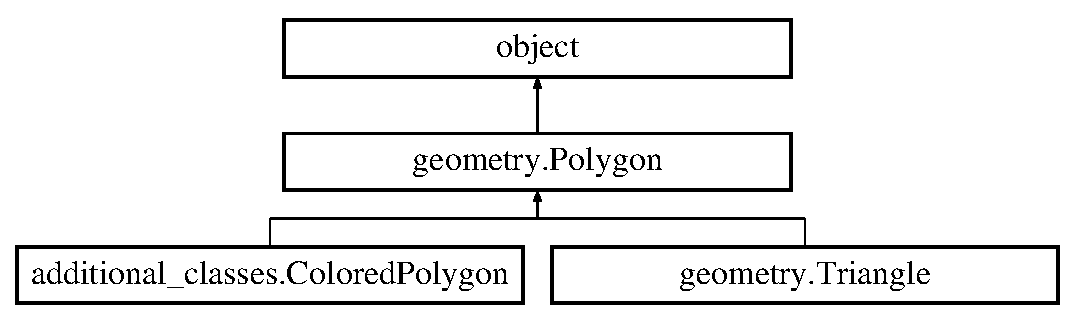
\includegraphics[height=3.000000cm]{classgeometry_1_1Polygon}
\end{center}
\end{figure}
\subsection*{Public Member Functions}
\begin{DoxyCompactItemize}
\item 
def \hyperlink{classgeometry_1_1Polygon_a46b21b7c846c26d6ff1171cc9a29d0c5}{\+\_\+\+\_\+init\+\_\+\+\_\+} (self, \hyperlink{classgeometry_1_1Polygon_aa0fda1ff74a09b8498bd7d8731b2fbf1}{points})
\item 
def \hyperlink{classgeometry_1_1Polygon_a9c05f0f70dbb5652e29265671b036c71}{\+\_\+\+\_\+repr\+\_\+\+\_\+} (self)
\item 
def \hyperlink{classgeometry_1_1Polygon_ac597f93df5686912dc1ca6eddc65b6b8}{\+\_\+\+\_\+hash\+\_\+\+\_\+} (self)
\item 
def \hyperlink{classgeometry_1_1Polygon_aa39e7d0353ffad956679321aca725d35}{comp\+Normal} (self)
\begin{DoxyCompactList}\small\item\em Calculating a Surface Normal for a triangle or a 3D polygon. \end{DoxyCompactList}\item 
def \hyperlink{classgeometry_1_1Polygon_a64880abb26797d5ad564a6f0399b216c}{contains} (self, p)
\item 
def \hyperlink{classgeometry_1_1Polygon_a4836c37e04dc0eb76809904538b77e7c}{is\+Convex} (self)
\item 
def \hyperlink{classgeometry_1_1Polygon_ae4ab82f837783f51b39a41427e46f5df}{does\+Line\+Cross\+Polygon} (self, line)
\item 
def \hyperlink{classgeometry_1_1Polygon_a4c6914db65978bbd2232f28bbb41b69b}{ccw} (self)
\end{DoxyCompactItemize}
\subsection*{Public Attributes}
\begin{DoxyCompactItemize}
\item 
\mbox{\Hypertarget{classgeometry_1_1Polygon_a4491c008a2f035119ca3f56d38afd0cf}\label{classgeometry_1_1Polygon_a4491c008a2f035119ca3f56d38afd0cf}} 
\hyperlink{classgeometry_1_1Polygon_a4491c008a2f035119ca3f56d38afd0cf}{n}
\begin{DoxyCompactList}\small\item\em number of vertices \end{DoxyCompactList}\item 
\mbox{\Hypertarget{classgeometry_1_1Polygon_aa0fda1ff74a09b8498bd7d8731b2fbf1}\label{classgeometry_1_1Polygon_aa0fda1ff74a09b8498bd7d8731b2fbf1}} 
\hyperlink{classgeometry_1_1Polygon_aa0fda1ff74a09b8498bd7d8731b2fbf1}{points}
\begin{DoxyCompactList}\small\item\em list of indexes of vertices \end{DoxyCompactList}\item 
\mbox{\Hypertarget{classgeometry_1_1Polygon_a904adb19928f3de57ee46d4410c527e3}\label{classgeometry_1_1Polygon_a904adb19928f3de57ee46d4410c527e3}} 
\hyperlink{classgeometry_1_1Polygon_a904adb19928f3de57ee46d4410c527e3}{normal}
\begin{DoxyCompactList}\small\item\em normal vector of the given polygon \end{DoxyCompactList}\end{DoxyCompactItemize}


\subsection{Detailed Description}
In elementary geometry, a polygon is a plane figure that is bounded by a finite chain of straight line segments, closing in a loop, to form a closed polygonal chain or circuit. 

These segments are called its edges or sides, and the points where two edges meet are the polygon\textquotesingle{}s vertices (singular\+: vertex) or corners. \begin{DoxyVerb}A class representing a polygon.\end{DoxyVerb}
 

Definition at line 354 of file geometry.\+py.



\subsection{Constructor \& Destructor Documentation}
\mbox{\Hypertarget{classgeometry_1_1Polygon_a46b21b7c846c26d6ff1171cc9a29d0c5}\label{classgeometry_1_1Polygon_a46b21b7c846c26d6ff1171cc9a29d0c5}} 
\index{geometry\+::\+Polygon@{geometry\+::\+Polygon}!\+\_\+\+\_\+init\+\_\+\+\_\+@{\+\_\+\+\_\+init\+\_\+\+\_\+}}
\index{\+\_\+\+\_\+init\+\_\+\+\_\+@{\+\_\+\+\_\+init\+\_\+\+\_\+}!geometry\+::\+Polygon@{geometry\+::\+Polygon}}
\subsubsection{\texorpdfstring{\+\_\+\+\_\+init\+\_\+\+\_\+()}{\_\_init\_\_()}}
{\footnotesize\ttfamily def geometry.\+Polygon.\+\_\+\+\_\+init\+\_\+\+\_\+ (\begin{DoxyParamCaption}\item[{}]{self,  }\item[{}]{points }\end{DoxyParamCaption})}

\begin{DoxyVerb}Constructor. Throws an exception if less than three points are given.\end{DoxyVerb}
 

Definition at line 357 of file geometry.\+py.



\subsection{Member Function Documentation}
\mbox{\Hypertarget{classgeometry_1_1Polygon_ac597f93df5686912dc1ca6eddc65b6b8}\label{classgeometry_1_1Polygon_ac597f93df5686912dc1ca6eddc65b6b8}} 
\index{geometry\+::\+Polygon@{geometry\+::\+Polygon}!\+\_\+\+\_\+hash\+\_\+\+\_\+@{\+\_\+\+\_\+hash\+\_\+\+\_\+}}
\index{\+\_\+\+\_\+hash\+\_\+\+\_\+@{\+\_\+\+\_\+hash\+\_\+\+\_\+}!geometry\+::\+Polygon@{geometry\+::\+Polygon}}
\subsubsection{\texorpdfstring{\+\_\+\+\_\+hash\+\_\+\+\_\+()}{\_\_hash\_\_()}}
{\footnotesize\ttfamily def geometry.\+Polygon.\+\_\+\+\_\+hash\+\_\+\+\_\+ (\begin{DoxyParamCaption}\item[{}]{self }\end{DoxyParamCaption})}

\begin{DoxyVerb}The hash is a tuple of all points sorted on x.\end{DoxyVerb}
 

Definition at line 380 of file geometry.\+py.

\mbox{\Hypertarget{classgeometry_1_1Polygon_a9c05f0f70dbb5652e29265671b036c71}\label{classgeometry_1_1Polygon_a9c05f0f70dbb5652e29265671b036c71}} 
\index{geometry\+::\+Polygon@{geometry\+::\+Polygon}!\+\_\+\+\_\+repr\+\_\+\+\_\+@{\+\_\+\+\_\+repr\+\_\+\+\_\+}}
\index{\+\_\+\+\_\+repr\+\_\+\+\_\+@{\+\_\+\+\_\+repr\+\_\+\+\_\+}!geometry\+::\+Polygon@{geometry\+::\+Polygon}}
\subsubsection{\texorpdfstring{\+\_\+\+\_\+repr\+\_\+\+\_\+()}{\_\_repr\_\_()}}
{\footnotesize\ttfamily def geometry.\+Polygon.\+\_\+\+\_\+repr\+\_\+\+\_\+ (\begin{DoxyParamCaption}\item[{}]{self }\end{DoxyParamCaption})}

\begin{DoxyVerb}String representation of this polygon.\end{DoxyVerb}
 

Definition at line 370 of file geometry.\+py.

\mbox{\Hypertarget{classgeometry_1_1Polygon_a4c6914db65978bbd2232f28bbb41b69b}\label{classgeometry_1_1Polygon_a4c6914db65978bbd2232f28bbb41b69b}} 
\index{geometry\+::\+Polygon@{geometry\+::\+Polygon}!ccw@{ccw}}
\index{ccw@{ccw}!geometry\+::\+Polygon@{geometry\+::\+Polygon}}
\subsubsection{\texorpdfstring{ccw()}{ccw()}}
{\footnotesize\ttfamily def geometry.\+Polygon.\+ccw (\begin{DoxyParamCaption}\item[{}]{self }\end{DoxyParamCaption})}

\begin{DoxyVerb}Returns True if the points are provided in CCW order.\end{DoxyVerb}
 

Definition at line 454 of file geometry.\+py.

\mbox{\Hypertarget{classgeometry_1_1Polygon_aa39e7d0353ffad956679321aca725d35}\label{classgeometry_1_1Polygon_aa39e7d0353ffad956679321aca725d35}} 
\index{geometry\+::\+Polygon@{geometry\+::\+Polygon}!comp\+Normal@{comp\+Normal}}
\index{comp\+Normal@{comp\+Normal}!geometry\+::\+Polygon@{geometry\+::\+Polygon}}
\subsubsection{\texorpdfstring{comp\+Normal()}{compNormal()}}
{\footnotesize\ttfamily def geometry.\+Polygon.\+comp\+Normal (\begin{DoxyParamCaption}\item[{}]{self }\end{DoxyParamCaption})}



Calculating a Surface Normal for a triangle or a 3D polygon. 

A surface normal for a triangle can be calculated by taking the vector cross product of two edges of that triangle. The order of the vertices used in the calculation will affect the direction of the normal (in or out of the face w.\+r.\+t. winding). Also you can use a Newell\textquotesingle{}s method for an arbitrary 3D polygon.

\begin{DoxyReturn}{Returns}
normal. 
\end{DoxyReturn}
\begin{DoxySeeAlso}{See also}
\href{https://www.khronos.org/opengl/wiki/Calculating_a_Surface_Normal}{\tt https\+://www.\+khronos.\+org/opengl/wiki/\+Calculating\+\_\+a\+\_\+\+Surface\+\_\+\+Normal} \begin{DoxyVerb}Newell's method for getting polygon normal.\end{DoxyVerb}
 
\end{DoxySeeAlso}


Definition at line 394 of file geometry.\+py.

\mbox{\Hypertarget{classgeometry_1_1Polygon_a64880abb26797d5ad564a6f0399b216c}\label{classgeometry_1_1Polygon_a64880abb26797d5ad564a6f0399b216c}} 
\index{geometry\+::\+Polygon@{geometry\+::\+Polygon}!contains@{contains}}
\index{contains@{contains}!geometry\+::\+Polygon@{geometry\+::\+Polygon}}
\subsubsection{\texorpdfstring{contains()}{contains()}}
{\footnotesize\ttfamily def geometry.\+Polygon.\+contains (\begin{DoxyParamCaption}\item[{}]{self,  }\item[{}]{p }\end{DoxyParamCaption})}

\begin{DoxyVerb}Returns True if p is inside this polygon.

   @see http://geomalgorithms.com/a03-_inclusion.html
\end{DoxyVerb}
 

Definition at line 407 of file geometry.\+py.

\mbox{\Hypertarget{classgeometry_1_1Polygon_ae4ab82f837783f51b39a41427e46f5df}\label{classgeometry_1_1Polygon_ae4ab82f837783f51b39a41427e46f5df}} 
\index{geometry\+::\+Polygon@{geometry\+::\+Polygon}!does\+Line\+Cross\+Polygon@{does\+Line\+Cross\+Polygon}}
\index{does\+Line\+Cross\+Polygon@{does\+Line\+Cross\+Polygon}!geometry\+::\+Polygon@{geometry\+::\+Polygon}}
\subsubsection{\texorpdfstring{does\+Line\+Cross\+Polygon()}{doesLineCrossPolygon()}}
{\footnotesize\ttfamily def geometry.\+Polygon.\+does\+Line\+Cross\+Polygon (\begin{DoxyParamCaption}\item[{}]{self,  }\item[{}]{line }\end{DoxyParamCaption})}

\begin{DoxyVerb}Returns whether this polygon is crossed by a given line.\end{DoxyVerb}
 

Definition at line 449 of file geometry.\+py.

\mbox{\Hypertarget{classgeometry_1_1Polygon_a4836c37e04dc0eb76809904538b77e7c}\label{classgeometry_1_1Polygon_a4836c37e04dc0eb76809904538b77e7c}} 
\index{geometry\+::\+Polygon@{geometry\+::\+Polygon}!is\+Convex@{is\+Convex}}
\index{is\+Convex@{is\+Convex}!geometry\+::\+Polygon@{geometry\+::\+Polygon}}
\subsubsection{\texorpdfstring{is\+Convex()}{isConvex()}}
{\footnotesize\ttfamily def geometry.\+Polygon.\+is\+Convex (\begin{DoxyParamCaption}\item[{}]{self }\end{DoxyParamCaption})}

\begin{DoxyVerb}Returns whether this polygon is convex.\end{DoxyVerb}
 

Definition at line 431 of file geometry.\+py.



The documentation for this class was generated from the following file\+:\begin{DoxyCompactItemize}
\item 
geometry.\+py\end{DoxyCompactItemize}

\hypertarget{classadditional__classes_1_1TemporaryLine}{}\section{additional\+\_\+classes.\+Temporary\+Line Class Reference}
\label{classadditional__classes_1_1TemporaryLine}\index{additional\+\_\+classes.\+Temporary\+Line@{additional\+\_\+classes.\+Temporary\+Line}}


Class that defines a temporary line (used to draw the temporary lines representing the polygon edges)  


\subsection*{Public Member Functions}
\begin{DoxyCompactItemize}
\item 
\mbox{\Hypertarget{classadditional__classes_1_1TemporaryLine_a5877e242c9aa50bdb7e97e343aad3d86}\label{classadditional__classes_1_1TemporaryLine_a5877e242c9aa50bdb7e97e343aad3d86}} 
def \hyperlink{classadditional__classes_1_1TemporaryLine_a5877e242c9aa50bdb7e97e343aad3d86}{\+\_\+\+\_\+init\+\_\+\+\_\+} (self, point)
\begin{DoxyCompactList}\small\item\em The constructor. \end{DoxyCompactList}\end{DoxyCompactItemize}
\subsection*{Public Attributes}
\begin{DoxyCompactItemize}
\item 
\mbox{\Hypertarget{classadditional__classes_1_1TemporaryLine_adba70ff80ce45632da0995384bee8fdb}\label{classadditional__classes_1_1TemporaryLine_adba70ff80ce45632da0995384bee8fdb}} 
{\bfseries start\+Point}
\item 
\mbox{\Hypertarget{classadditional__classes_1_1TemporaryLine_a94c00c5880ba274d4fecfd43bc45b657}\label{classadditional__classes_1_1TemporaryLine_a94c00c5880ba274d4fecfd43bc45b657}} 
{\bfseries end\+Point}
\end{DoxyCompactItemize}


\subsection{Detailed Description}
Class that defines a temporary line (used to draw the temporary lines representing the polygon edges) 

Definition at line 54 of file additional\+\_\+classes.\+py.



The documentation for this class was generated from the following file\+:\begin{DoxyCompactItemize}
\item 
additional\+\_\+classes.\+py\end{DoxyCompactItemize}

\hypertarget{classgeometry_1_1Triangle}{}\section{geometry.\+Triangle Class Reference}
\label{classgeometry_1_1Triangle}\index{geometry.\+Triangle@{geometry.\+Triangle}}


A triangle is a polygon with three edges and three vertices.  


Inheritance diagram for geometry.\+Triangle\+:\begin{figure}[H]
\begin{center}
\leavevmode
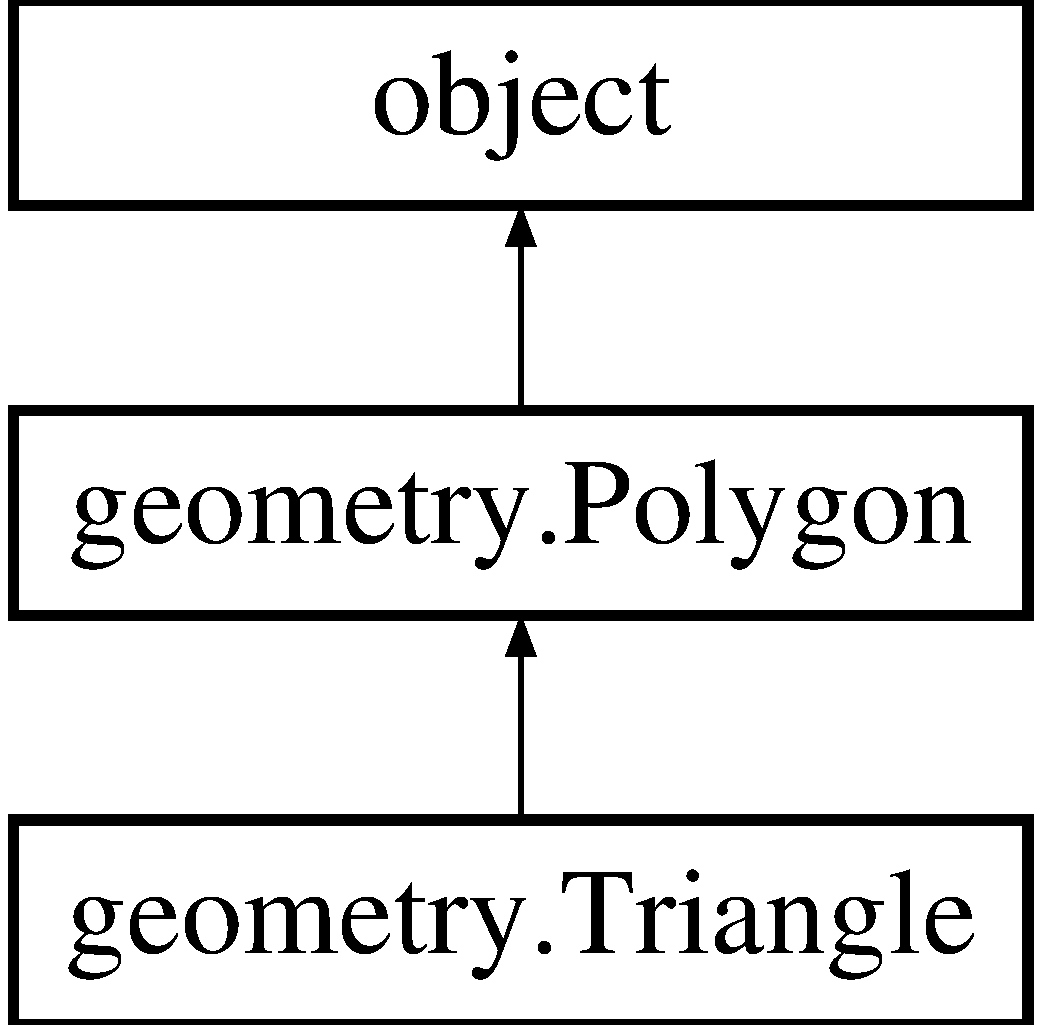
\includegraphics[height=3.000000cm]{classgeometry_1_1Triangle}
\end{center}
\end{figure}
\subsection*{Public Member Functions}
\begin{DoxyCompactItemize}
\item 
\mbox{\Hypertarget{classgeometry_1_1Triangle_a4e7dfc53b80ea22d888ed43d9b401cf5}\label{classgeometry_1_1Triangle_a4e7dfc53b80ea22d888ed43d9b401cf5}} 
def {\bfseries \+\_\+\+\_\+init\+\_\+\+\_\+} (self, A, B, C)
\item 
def \hyperlink{classgeometry_1_1Triangle_aefd0596cf3d91438d5214c303d426bc6}{area} (self)
\item 
def \hyperlink{classgeometry_1_1Triangle_a714f4af89b1855e957797e2c53568893}{interior\+Point} (self)
\end{DoxyCompactItemize}
\subsection*{Additional Inherited Members}


\subsection{Detailed Description}
A triangle is a polygon with three edges and three vertices. 

It is one of the basic shapes in geometry. A triangle with vertices A, B, and C is denoted △ A B C.

Three non-\/collinear points define a unique triangle and a unique plane.\begin{DoxyVerb}Just a triangle, the simplest polygon possible.\end{DoxyVerb}
 

Definition at line 551 of file geometry.\+py.



\subsection{Member Function Documentation}
\mbox{\Hypertarget{classgeometry_1_1Triangle_aefd0596cf3d91438d5214c303d426bc6}\label{classgeometry_1_1Triangle_aefd0596cf3d91438d5214c303d426bc6}} 
\index{geometry\+::\+Triangle@{geometry\+::\+Triangle}!area@{area}}
\index{area@{area}!geometry\+::\+Triangle@{geometry\+::\+Triangle}}
\subsubsection{\texorpdfstring{area()}{area()}}
{\footnotesize\ttfamily def geometry.\+Triangle.\+area (\begin{DoxyParamCaption}\item[{}]{self }\end{DoxyParamCaption})}

\begin{DoxyVerb}Returns triangle area.\end{DoxyVerb}
 

Definition at line 557 of file geometry.\+py.

\mbox{\Hypertarget{classgeometry_1_1Triangle_a714f4af89b1855e957797e2c53568893}\label{classgeometry_1_1Triangle_a714f4af89b1855e957797e2c53568893}} 
\index{geometry\+::\+Triangle@{geometry\+::\+Triangle}!interior\+Point@{interior\+Point}}
\index{interior\+Point@{interior\+Point}!geometry\+::\+Triangle@{geometry\+::\+Triangle}}
\subsubsection{\texorpdfstring{interior\+Point()}{interiorPoint()}}
{\footnotesize\ttfamily def geometry.\+Triangle.\+interior\+Point (\begin{DoxyParamCaption}\item[{}]{self }\end{DoxyParamCaption})}

\begin{DoxyVerb}Returns a random point into triangle.\end{DoxyVerb}
 

Definition at line 565 of file geometry.\+py.



The documentation for this class was generated from the following file\+:\begin{DoxyCompactItemize}
\item 
geometry.\+py\end{DoxyCompactItemize}

%--- End generated contents ---

% Index
\backmatter
\newpage
\phantomsection
\clearemptydoublepage
\addcontentsline{toc}{chapter}{Index}
\printindex

\end{document}
